\chapter{Conifer Broadleaf Forest: Vines, Epiphytes and Parasites}

Woody and herbaceous vines, vascular epiphytes or `perching plants', and vascular parasites and saprophytes are abundant and distinctive features of tropical rain forests.\footnote{\cite{richards1952tropical}}
The stems of the vines climb their supports by a variety of means, including twining of the stems, tendrils, hooks and attaching roots.
The epiphytes range from herbaceous plants to large trees.
Among the former are nest epiphytes, with their large leaf rosettes, and an abundance of orchids, and among the latter are the `strangling' epiphytes, including many species of fig (\BotanicRef{Ficus}).
The parasites attack stems or roots and may be without chlorophyll and completely parasitic or with chlorophyll and so able to manufacture some of their food requirements.
Saprophytes are devoid of chlorophyll and are thought to derive their energy requirements from decaying organic material, particularly leaf litter, on the forest floor.

Surprisingly, in view of our temperate latitudes, a comparable range of vines and epiphytes are equally conspicuous in the New Zealand conifer broadleaf forest, but these have received little attention in books on New Zealand forest plants for the general reader.
This partial neglect is perhaps understandable, as it is not easy to get close to the foliage, flowers and fruits of many of these plants, particularly where they occur high in the branches of tall trees.
Binoculars help, but few botanists are as intrepid as J. L. Harrison-Smith,\footnote{\cite{harrisonsmith1938kauri}} who spent many hours `wandering about' among the branches of giant \IDX{kauri}s recording epiphytes.
In his own words:

\begin{quote}
	In order to catalogue the plants the trees were climbed.
	Ordinary gum collectors' climbing gear (spiked boots and climbing hooks) were used.
	Descent was accomplished with a bosun's chair suspended from a rope.
	It was then possible to examine the trunk and any isolated branches on the way down.
\end{quote}

Fortunately it is possible to reach most vines and epiphytes without taking such risks.
Some species grow low on the trunks of trees and so are readily accessible, but even those normally restricted to tree crowns may descend to lower levels in well-lit situations and, in the normal course of events, trees are blown or fall over\figureref{\fullref{fig:26kahikatea}} and then a full range of high epiphytes and vines, albeit somewhat damaged, can be examined.

\begin{SCfigure}[1.0][htb]
	\centering
	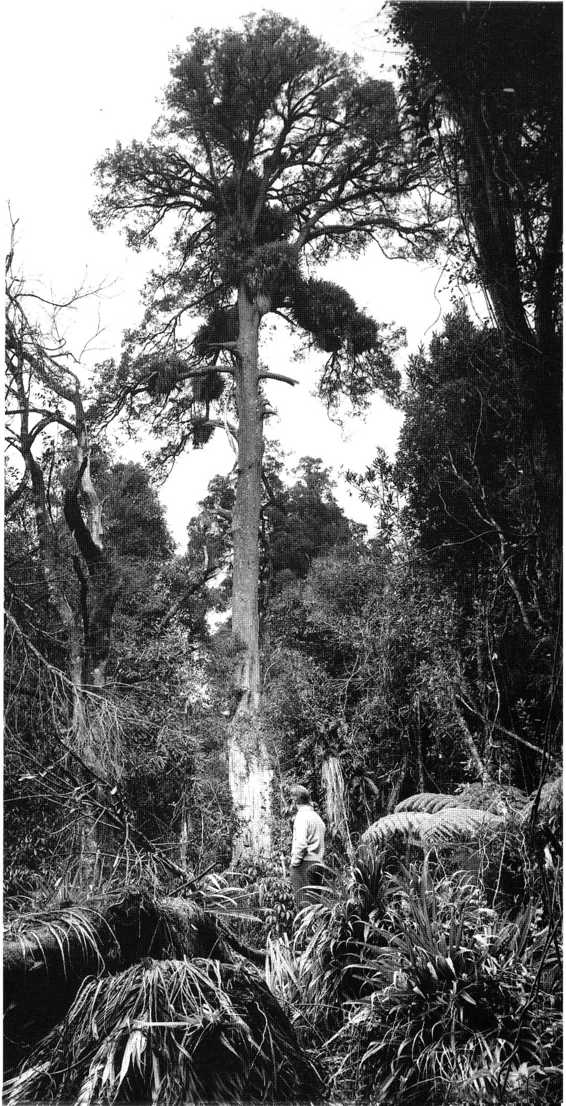
\includegraphics[width=0.5\textwidth]{graphics/figure26kahikatea.jpg}
	\caption[Kahikatea with asteliad nest epiphytes]{Kahikatea (\BotanicRef{Dacrycarpus dacrydioides}[Dacrycarpus][dacrydioides]) with asteliad nest epiphytes.
	The tree originally had two trunks.
	The nearest one has fallen and its crown and epiphytes can be seen in the foreground.
	Te Marua near Wellington, southern North Island.
	Photo: M. D. King}%
	\label{fig:26kahikatea}
\end{SCfigure}

Not infrequently the categories of vines, epiphytes and parasites are confused, so that if it is stated that a plant `grows epiphytically on trees', further enquiry is often necessary to determine the precise mode of growth of the species in question.
It is true that the word `epiphyte', meaning `a plant that grows on other plants', fits all three categories, but as in other respects their life styles are quite distinct, this term should be restricted to plants which germinate and establish themselves on the trunk and branch surfaces of trees.
Vines, by contrast, establish themselves on the ground, then grow up the trees.
Some parasites are similar to epiphytes in that their seeds germinate on trunks and branches, but they differ markedly in having special root-like organs that penetrate the living tissues of their host and draw water and nutrients from them.

\section{Vines --- Subcanopy Climbers}

Vines in this category are herbaceous and attach themselves to tree trunks by special roots arising from the stems.
They ascend for varying distances up the trunks, but mostly do not enter the tree crowns.
They are all able to reproduce in the reduced light of the forest interior.

\begin{figure}[htb]
	% Outer minipage scaled to limit width.
	% Inner minipages scaled so the images have the same height.
	\begin{minipage}[t]{0.7\textwidth}
		\begin{minipage}[t]{(\textwidth-\fgap) * \real{0.496}}
			\centering
			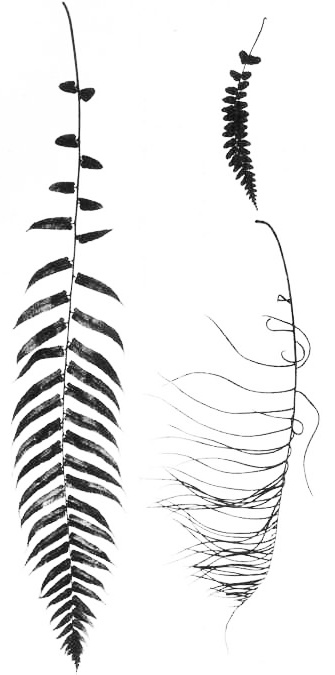
\includegraphics[width=\textwidth]{graphics/figure27fern.jpg}
			\caption[Leaves of the climbing fern \emph{Blechnum filiforme}]{Leaves of the climbing fern \BotanicRef{Blechnum filiforme}[Blechnum][filiforme].
			Top right, a small leaf from the base of a tree trunk.
			Left, large leaf from \SI{2}{\metre} above ground level.
			Lower right, fertile leaf.
			Photo: M. D. King.}%
			\label{fig:27fern}
		\end{minipage}\hspace{\fgap}%
		\begin{minipage}[t]{(\textwidth-\fgap) * \real{0.504}}
			\centering
			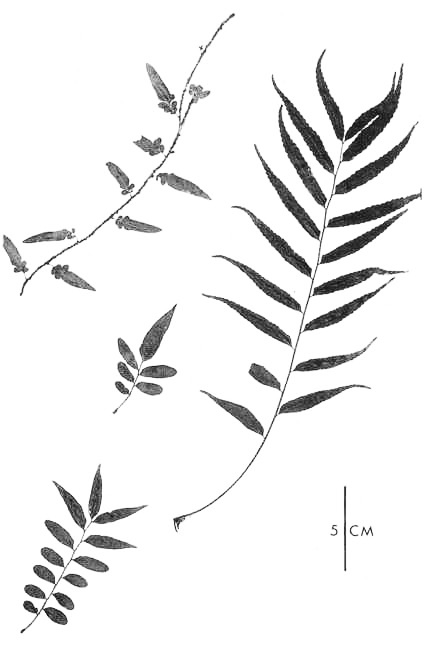
\includegraphics[width=\textwidth]{graphics/figure28fern.jpg}
			\caption[Leaves of the climbing fern \emph{Arthropteris tenella}]{Leaves of the climbing fern \BotanicRef{Arthropteris tenella}[Arthropteris][tenella].
			Top left, climbing stem with small juvenile leaves.
			Top right, large adult leaf.
			The other leaves are at intermediate stages.
			Photo  J. E. Casey.}%
			\label{fig:28fern}
		\end{minipage}
	\end{minipage}
\end{figure}

In New Zealand all vines in this category are ferns and in some, as in the climbing members of the arum lily family in the tropics, there is a remarkable increase in size and complexity of the leaves as their height above the ground increases.
The best known example of this is \BotanicRef{Blechnum filiforme}[Blechnum][filiforme]\figureref{\fullref{fig:27fern}}, a common plant in lowland forest as far south as the northern South Island. \BotanicRef{Blechnum filiforme}[Blechnum][filiforme] is often abundant on the forest floor where it spreads by slender rhizomes.\footnote{Rhizomes are horizontal stems on or below the surface of a substrate, usually the ground.}
In this situation the leaves are only about \SI{10}{\centi\metre} long and once-pinnate, with leaflets which range in shape from small and oblong to almost round.
Where the stems grow up tree trunks, as they frequently do, the leaves produced become progressively larger, until several metres above the ground they attain a maximum length of almost \SI{35}{\centi\metre} and have long, narrow, pointed leaflets up to \SI{10}{\centi\metre} long.
It is among these largest leaves that the fertile, spore-bearing fronds, with their almost threadlike leaflets, are produced.
The leaves of this species are dark-green and fairly thin.
The climbing stems branch and the branches tend to stay close together and grow more or less vertically, sometimes reaching as high as \SI{10}{\metre} above the ground.

\BotanicRef{Arthropteris tenella}[Arthropteris][tenella]\figureref{\fullref{fig:28fern}} also has relatively thin, dark leaves and slender, vertically ascending stems, but these generally reach to only a few metres above the ground.
This species also reaches the northern South Island, but is less common than \BotanicRef{Blechnum filiforme}[Blechnum][filiforme] and is mostly encountered in coastal forests and some low altitude inland locations.
The juvenile leaves are \SIrange{5}{10}{\centi\metre} long, once-pinnate and often rather peculiar in appearance --- the few pairs of lateral leaflets are small and almost circular; the terminal leaflet is much larger and longer, narrowing to a point.
Fully adult leaves are \SI{30}{\centi\metre} or more long with many pairs of narrow, wavy-margined leaflets up to \SI{8}{\centi\metre} long.

\begin{SCfigure}[1.5][htb]
	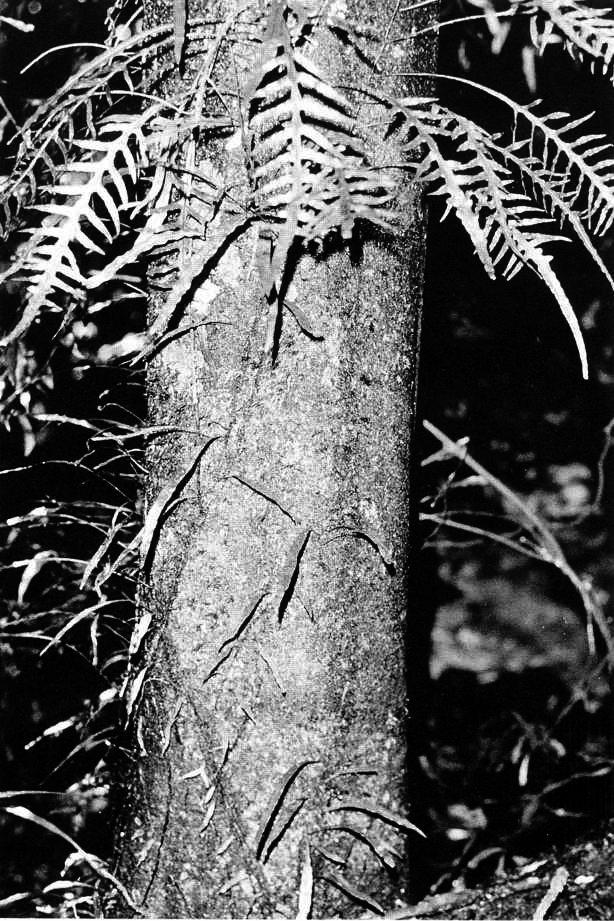
\includegraphics[width=0.4\textwidth]{graphics/figure29scandens.jpg}
	\centering
	\caption[\emph{Phymatosorus scandens} growing up a tree trunk]{\BotanicRef{Phymatosorus scandens}[Phymatosorus][scandens] growing up a tree trunk.
The simple leaves are juvenile and compound leaves adult.
	Photo: J. E. Casey.}%
	\label{fig:29scandens}
\end{SCfigure}

The light green, thin-leaved \BotanicRef{Phymatosorus scandens}[Phymatosorus][scandens] also shows a trend from juvenile to adult leaves with increasing height\figureref{\fullref{fig:29scandens}}, but in this case the juveniles are about as long as the adults, up to \SI{35}{\centi\metre}, but are narrow, undivided and usually sterile.
There is often a fairly abrupt change to the adult leaves, which are much wider and are deeply incised into a number of narrow, lateral segments bearing sporangia.\footnote{Sporangia are organs containing spores.}
This species often occurs with \BotanicRef{Blechnum filiforme}[Blechnum][filiforme] in lowland forests, sometimes on the same tree, but it ranges further to the south of the South Island.
It is able to climb vertical tree trunks with its slender stems spreading in various directions, but it does not often attain the heights of \BotanicRef{Blechnum filiforme}[Blechnum][filiforme].

The thick-leaved \BotanicRef{Phymatosorus diversifolius}[Phymatosorus][diversifolius], with its stout, grey-green, black-flecked stems, is better known to most people.
It ascends to higher altitudes than the species so far considered and also reaches the Auckland Islands to the south of New Zealand.
It differs too in often preferring to climb inclined trunks and inclined or horizontal branches, so it is most common on trees such as \IDX{mahoe}, tree \BotanicRef{Fuchsia} and \IDX{kamahi}, all of which have short trunks and many spreading branches.
This fern may extend along all the branches and eventually into the crown of such trees.
The stems branch freely and often rather untidily on their supports, sometimes curving completely around them.
Where \BotanicRef{Phymatosorus diversifolius}[Phymatosorus][diversifolius] grows on the upper sides of more or less horizontal branches, quite a thick layer of humus builds up beneath its stems.

As the name of this species indicates, it has a range of leaf forms similar to \BotanicRef{Phymatosorus scandens}[Phymatosorus][scandens].\footnote{Synomyms \BotanicRef{Dendroconche scandens}[Dendroconche][scandens], \BotanicRef{Microsorum scandens}[Microsorum][scandens].}
On a tree with a heavy growth of the fern, the large, shiny, bright green leaves are rather widely spaced and deeply incised into narrow segments with an abundance of sporangia beneath, aggregated into distinctive orange spots or sori.
Young plants establishing themselves in moss on trunk bases have narrow, undivided sterile leaves. \BotanicRef{Phymatosorus diversifolius}[Phymatosorus][diversifolius] also grows on the ground, most abundantly on rocky slopes.
In rocky, exposed places the narrow, undivided leaves may persist, but in these circumstances they bear sporangia.

A third species of \BotanicRef{Phymatosorus} --- \BotanicRef{Phymatosorus novae-zelandiae}[Phymatosorus][novae-zelandiae] --- is found in montane forests throughout the North Island, but is absent from the South Island.
With its stout rhizomes it is similar to \BotanicRef{Phymatosorus diversifolius}[Phymatosorus][diversifolius], but the rhizomes are densely covered with straw-coloured scales and the leaves are generally larger with more numerous, narrower and longer lateral segments.
It appears that there are no marked variations in leaf form in this species.

\BotanicRef{Rumohra adiantiformis}[Rumohra][adiantiformis] ranges throughout New Zealand in lowland to montane forests and is most common as a climber on tree fern trunks.
The much divided leaves have a leathery texture and bear conspicuous black sori.
There is a modest increase in the size of leaves with increasing height.

Filmy ferns may be common as climbers in high rainfall areas.
In some cases the fronds are very small and delicate and grow intermingled with mosses, but some species --- \BotanicRef{Hymenophyllum dilatation}[Hymenophyllum][dilatation], \BotanicRef{Hymenophyllum scabrum}[Hymenophyllum][scabrum], \BotanicRef{Hymenophyllum sanguinolentum}[Hymenophyllum][sanguinolentum] and several others --- have relatively large leaves which, Holloway\footnote{\cite{holloway1923studies}} notes, increase in size with increasing height above the ground.
Holloway suggests that the increased leaf areas enable more effective absorption of water by the thin leaves in the drier tree trunk habitat.
The \IDX{kidney fern} (\BotanicRef{Trichomanes reniforme}[Trichomanes][reniforme]) is perhaps our most unusual filmy fern.
Its leaves are undivided and, as both common and botanical names indicate, kidney-shaped.
This fern usually grows for only a short distance up tree trunks, but can climb much higher in moist situations.
A strange case is the densely hairy \BotanicRef{Hymenophyllum malingii}[Hymenophyllum][malingii], which climbs on the dead trunks of trees, particularly mountain cedar (\BotanicRef{Libocedrus bidwillii}[Libocedrus][bidwillii]).
The climbing species of filmy fern range throughout the country.

Six of the climbing ferns considered here are restricted to New Zealand.
The ranges of others are:

\BotanicRef{Phymatosorus diversifolius}[Phymatosorus][diversifolius]: Australia, Tasmania, tropical Polynesia.

\BotanicRef{Phymatosorus scandens}[Phymatosorus][scandens]: Australia, Norfolk Island.

\BotanicRef{Arthropteris tenella}[Arthropteris][tenella]: Australia, Norfolk Island, \IDX{New Caledonia}.

\BotanicRef{Rumohra adiantiformis}[Rumohra][adiantiformis]: South temperate zone, tropical Polynesia, tropical America.

\section{Canopy Climbers}

Vines whose foliage eventually spreads into the canopy of the forest are usually woody and are often referred to as lianes.\footnote{\cite{bird1916observations}}
At the adult stage they are light-demanding and generally produce flowers, or spores, only in well-lit situations.
Young plants on the forest floor are more shade-tolerant, but nevertheless establish most abundantly in the better lit earlier stages in forest development or in canopy gaps in mature forest.
Unlike the sub-canopy climbers, the lianes climb by a variety of means --- attaching roots, twining stems, hooks and tendrils.

\subsection{Root Climbers}

\begin{figure}[!htb]
	% Outer minipage scaled to limit width.
	% Inner minipages scaled so the images have the same height.
	\begin{minipage}[t]{0.9\textwidth}
		\begin{minipage}[t]{(\textwidth-\fgap) * \real{0.463}}
			\centering
			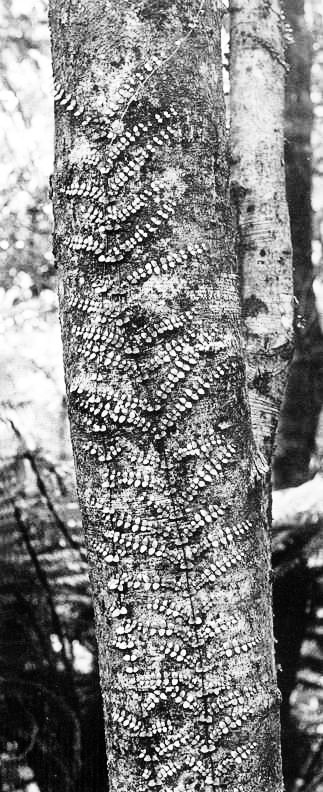
\includegraphics[width=\textwidth]{graphics/figure30rata.jpg}
			\caption[Young stage of white climbing rata]{Young stage of white climbing \IDX{rata} (\BotanicRef{Metrosideros perforata}[Metrosideros][perforata]) forming a leaf mosaic on a tree trunk. Photo: B. V. Sneddon.}%
			\label{fig:30rata}
		\end{minipage}\hspace{\fgap}%
		\begin{minipage}[t]{(\textwidth-\fgap) * \real{0.537}}
			\centering
			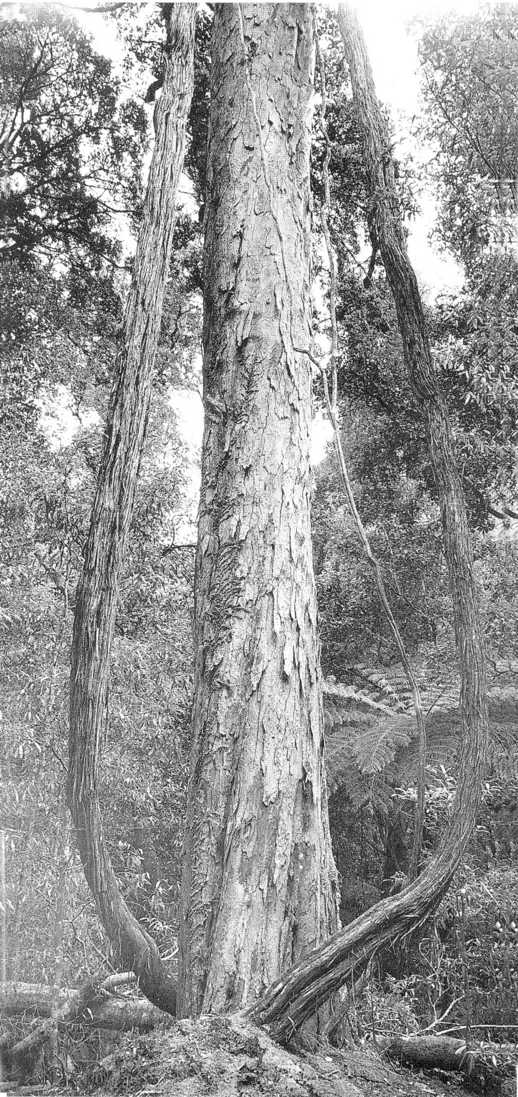
\includegraphics[width=\textwidth]{graphics/figure31perforata.jpg}
			\caption[A mature \emph{Metrosideros perforata} on a rimu]{The cable-like stems of a mature \BotanicRef{Metrosideros perforata}[Metrosideros][perforata] on a \IDX{rimu} (\BotanicRef{Dacrydium cupressinum}[Dacrydium][cupressinum]). Kaitoke, near Wellington, southern North Island. Photo: M. D. King.}%
			\label{fig:31perforata}
		\end{minipage}
	\end{minipage}
\end{figure}

The most prominent root climbers are the climbing \IDX{rata}s,\footnote{\cite{dawson1967growth}} currently included in the genus \BotanicRef{Metrosideros}.
They are able to grow up quite large trunks and are perhaps most abundant on the emergent conifers and the \IDX{northern rata}[rata!northern].
Their climbing stems are usually quite slender and the leaves, which form a close mosaic on the tree trunk\figureref{\fullref{fig:30rata}}, are generally smaller, thinner and more rounded than those of the adult stage.
When the stems reach full light high in the tree crown, or adequate light in the lower levels, they form a bushy growth of branches which extend away from the support and eventually bear flowers.
At this stage the stems extending up from the ground enlarge considerably and swing away from the host trunk as woody cables\figureref{\fullref{fig:31perforata}}. \BotanicRef{Metrosideros fulgens}[Metrosideros][fulgens] and \BotanicRef{Metrosideros perforata}[Metrosideros][perforata] form the largest stems, sometimes up to \SI{15}{\centi\metre} or more in diameter, but the others may attain \SIrange{7}{8}{\centi\metre}.
Often no leaves are visible near the ground, but the stems can be identified to some extent from the bark --- \BotanicRef{Metrosideros perforata}[Metrosideros][perforata] has red-brown stringy bark, \BotanicRef{Metrosideros fulgens}[Metrosideros][fulgens] also red-brown bark separating in thickish strips and the other species have pale whitish bark separating in thin flakes.

\BotanicRef{Metrosideros albiflora}[Metrosideros][albiflora] and \BotanicRef{Metrosideros carminea}[Metrosideros][carminea] are restricted to the northern North Island. \BotanicRef{Metrosideros albiflora}[Metrosideros][albiflora] is most common in \IDX{kauri forest}[kauri!forest]s.
It has the largest leaves of the group and small, white flowers. \BotanicRef{Metrosideros carminea}[Metrosideros][carminea] is much rnore colourful, with masses of large, crimson flowers, and it is now popular as a garden plant. \BotanicRef{Metrosideros perforata}[Metrosideros][perforata], \BotanicRef{Metrosideros fulgens}[Metrosideros][fulgens] and \BotanicRef{Metrosideros diffusa}[Metrosideros][diffusa] frequently occur together as far as the northern South Island and \BotanicRef{Metrosideros diffusa}[Metrosideros][diffusa] continues alone to Fiordland. \BotanicRef{Metrosideros diffusa}[Metrosideros][diffusa] often forms slender stems near the ground which spread widely in the humus of the forest floor and climb any trunks they encounter. \BotanicRef{Metrosideros colensoi}[Metrosideros][colensoi] also reaches the northern South Island, but is more localised in its occurrence, favouring forests on fertile soils such as those of river terraces.
The strongly weeping habit of its foliage is a distinctive feature. \BotanicRef{Metrosideros fulgens}[Metrosideros][fulgens] has large flowers ranging in colour from orange to dark red, while the other species have small white to pinkish flowers.
Most of the climbing \IDX{rata}s flower from early to mid-summer, but \BotanicRef{Metrosideros carminea}[Metrosideros][carminea] flowers in early spring and \BotanicRef{Metrosideros fulgens}[Metrosideros][fulgens] is remarkable both for the timing and length of its flowering season --- the first flowers may appear in late summer and flowering continues through the winter into early spring.

New Zealand is not the only place where climbing species of Metrosideros occur.
There are climbers related to ours in New Guinea and the Philippines.

The only other root climbing liane in New Zealand is the \IDX{kiekie} (\BotanicRef{Freycinetia baueriana var.\ banksii}[Freycinetia][baueriana var.\ banksii]).
It belongs to a distinctly tropical family, the Pandanaceae, which is represented by many species of \BotanicRef{Freycinetia} and \BotanicRef{Pandanus} in tropical rain forests.
One might expect that the outlying New Zealand species would be of reduced form and perhaps rare.
In fact it compares with the largest and most robust tropical species and is abundant in lowland, especially swampy forests as far as the south west of the South Island.
Tree trunks are often completely obscured by the foliage of \IDX{kiekie}\figureref{\fullref{fig:32kiekie}}, which can extend into the highest crowns \SI{30}{\metre} or more above the ground.
The leaves are dark green, narrow and a metre or more long with finely toothed cutting edges.
The male and female inflorescences found on separate plants are cone-like and surrounded by leaf-like white or purplish bracts, which are sweet and edible.
The stems are a few centimetres in diameter and distinctively ringed with leaf scars.
They give rise to slender, attaching roots, which branch freely towards their ends and attach themselves firmly to the trunk.
Other roots are stouter and grow down the trunk to the ground, often building up into quite thick and rather untidy masses.

\begin{figure}[htb]
	% Outer minipage scaled to limit width.
	% Inner minipages scaled so the images have the same height.
	\begin{minipage}[t]{\textwidth}
		\begin{minipage}[t]{(\textwidth-\fgap) * \real{0.512}}
			\centering
			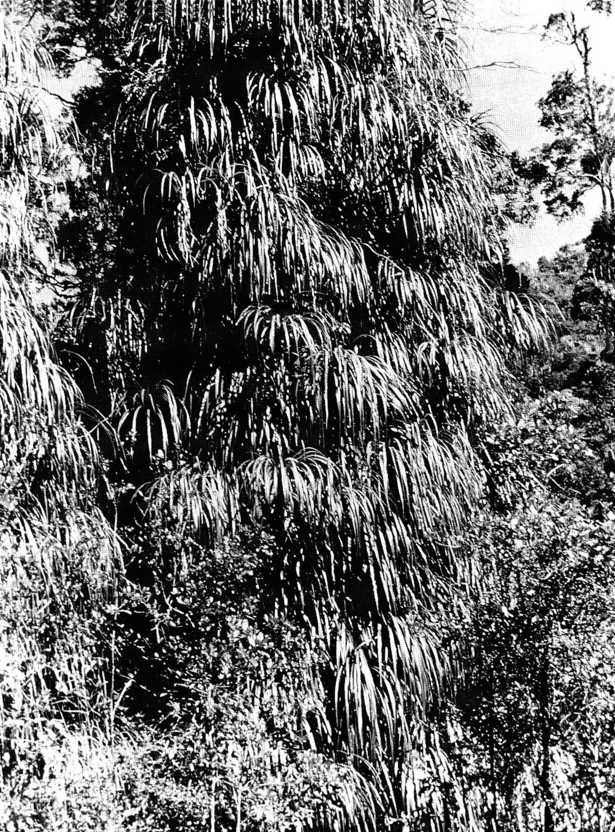
\includegraphics[width=\textwidth]{graphics/figure32kiekie.jpg}
			\caption[The drooping stems and foliage of kiekie]{The drooping stems and foliage of \IDX{kiekie} (\BotanicRef{Freycinetia baueriana var.\ banksii}[Freycinetia][baueriana var.\ banksii]) completely obscuring a \IDX{kahikatea} trunk. Kaitoke, near Wellington, southern North Island. Photo: J. W. Dawson.}%
			\label{fig:32kiekie}
		\end{minipage}\hspace{\fgap}%
		\begin{minipage}[t]{(\textwidth-\fgap) * \real{0.488}}
			\centering
			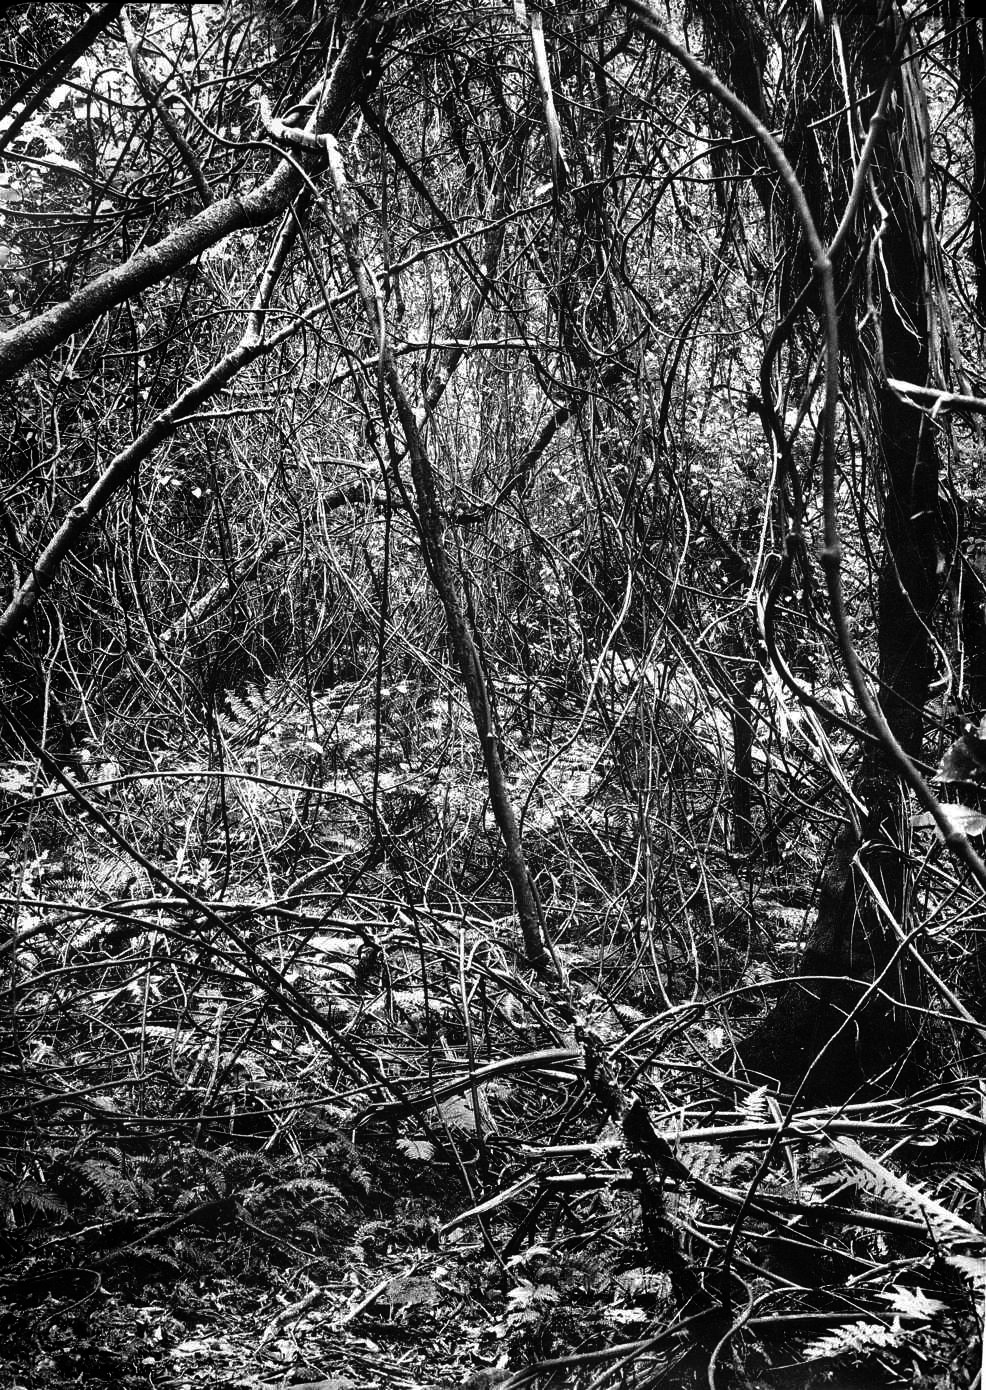
\includegraphics[width=\textwidth]{graphics/figure33supplejack.jpg}
			\caption[An entanglement of supplejack]{An entanglement of \IDX{supplejack} (\BotanicRef{Ripogonum scandens}[Ripogonum][scandens]). Photo:  M. D. King.}%
			\label{fig:33supplejack}
		\end{minipage}
	\end{minipage}
\end{figure}

\subsection{Twining Stem Climbers}

Twining lianes have climbing stems which wind around their supports in a clockwise or anticlockwise direction, depending on the species, until they reach the full light of the forest canopy.
Unlike root climbers, many twiners are not able to climb large tree trunks --- their turning circle is too small for that --- so they either have to climb young slender trees and grow with them into the canopy or climb small or young subcanopy trees and transfer from their crowns to those of taller trees.
Many twiners also climb stems of their own species which have already gained the forest roof.

Undoubtedly \IDX{supplejack} (\BotanicRef{Ripogonum scandens}[Ripogonum][scandens]), which ranges throughout the country, is the most familiar twiner in New Zealand forests,\footnote{\cite{macmillan1973biological}} particularly on alluvial and swampy sites.
It belongs to the lily family, taken in a wide sense, and its almost black, jointed, bamboo-like climbing stems often form entanglements that greatly impede progress\figureref{\fullref{fig:33supplejack}}.
Fortunately, unlike several of its relatives in Australia, \IDX{supplejack} does not have prickles.
Aggregations of woody, tuber-like rhizomes below ground give rise to the climbing stems which are dark-brown to black, \SIrange{1}{2}{\centi\metre} in diameter and which bear pairs of long narrow, often twisted scales in place of leaves.
The stem tips are reminiscent of \BotanicRef{Asparagus} and are soft and easily broken.
They can elongate at an average rate of \SI{5}{\centi\metre} per day in summer and while growing upwards the upper part of the shoot revolves slowly in an anticlockwise direction.
If it does not encounter a support it bends down to the ground and grows up again from the tip.

\IDX{Supplejack}[supplejack] mostly climbs fairly slender supports, but can also twine around quite large trunks, the record being a \IDX{kohekohe} of \SI{1.5}{\metre} diameter.\footnote{\cite{macmillan1973biological}}
When a climbing stem reaches the forest canopy, lateral climbing stems arise from its upper parts and eventually bear relatively slender, leafy stems of limited growth, which are unable to twine.
The leaves are broad and distinctively veined with two strong lateral veins more or less parallel to the midrib.
The leafy stems bear small flowers followed by bright red berries.
When lateral climbing stems are formed near the ground they are often swollen-and tuber-like at the base and produce roots which may descend more than a metre to the ground.
\IDX{Supplejack}[supplejack] is restricted to New Zealand, but other species of \BotanicRef{Ripogonum} are found in eastern Australia and New Guinea.

The two species of \BotanicRef{Parsonsia}, sometimes known as native jasmine, are found in lowland forest and shrubland throughout the country, \BotanicRef{Parsonsia heterophylla}[Parsonsia][heterophylla] is the larger of the two, with stems up to \SI{10}{\centi\metre} in diameter which attain heights up to \SI{20}{\metre} above the ground.
It is commonest near forest margins, but can reach the crowns of taller trees deeper in the forest by spreading from lower to higher levels in the forest canopy.

\begin{SCfigure}[1.0][htb]
	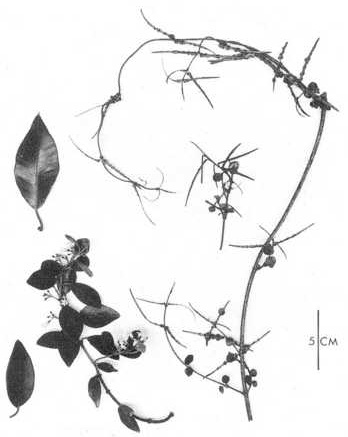
\includegraphics[width=0.5\textwidth]{graphics/figure34parsonsia.jpg}
	\centering
	\caption[The vine \emph{Parsonsia heterophylla}]{The vine \BotanicRef{Parsonsia heterophylla}[Parsonsia][heterophylla]. Juvenile foliage: right. Adult foliage and leaves: left. Photo: J. E. Casey.}%
	\label{fig:34parsonsia}
\end{SCfigure}

There is a very marked difference in size and shape between juvenile and adult leaves in this species\figureref{\fullref{fig:34parsonsia}}.
The seedlings establish themselves in sometimes quite shady places on the forest floor and the first few leaves produced are small and almost circular.
These are followed by leaves tending towards the second type of juvenile leaf, which is long and narrow with smooth or wavy margins.
Intermediates may be narrow at the base and round at the tip, or narrow at the base and tip and round in the middle, and, to make matters even more complicated, lateral branches on the seedlings usually repeat the same sequence.
The result is a bewildering and apparently random arrangement of leaf forms.
Some of the seedlings are completely green, others are largely brown and some leaves of the latter are unusually attractive with a mosaic of green, dark brown and pale brown patches.\footnote{This is a curious phenomenon also to be found in the equally variable leaves of juvenile \IDX{pokaka} (\BotanicRef{Elaeocarpus hookerianus}[Elaeocarpus][hookerianus]), juvenile \BotanicRef{Pittosporum obcordatum}[Pittosporum][obcordatum], seedling \IDX{lancewood} (\BotanicRef{Pseudopanax crassifolius}[Pseudopanax][crassifolius]) and others.}
The adult leaves, which are formed when the stems reach full light, are much larger and broader and generally uniform in shape, although there are often modest differences in shape between different vines.

The seedlings, which rotate in an anticlockwise direction at their tips as they grow upwards, reach about \SI{45}{\centi\metre} in height without support and somewhat higher if two or more seedlings twine about each other.
If no support is encountered then the stems bend down to the ground and grow along it until they find something to climb.
The supporting stems are usually slender, although \BotanicRef{Parsonsia heterophylla}[Parsonsia][heterophylla] has been observed climbing tree trunks of up to \SI{25}{\centi\metre} in diameter.

\BotanicRef{Parsonsia capsularis}[Parsonsia][capsularis] has small flowers, different in form from those of \BotanicRef{Parsonsia heterophylla}[Parsonsia][heterophylla], but the adult leaves of some varieties of the two species are very similar. \BotanicRef{Parsonsia capsularis}[Parsonsia][capsularis] also has long, narrow, reddish-brown juvenile leaves, and in some cases these are retained at the adult flowering stage.
This is a smaller plant than its more common relative and grows in shrub communities and, less often, at forest margins.
The small, fragrant flowers of these two species are borne in clusters and are white, yellow or, in the case of \BotanicRef{Parsonsia capsularis}[Parsonsia][capsularis] only, red.
The fruits are pod-like, hang downwards and split open to release numerous seeds, each with a dense tuft of hairs for wind dispersal.

The distinctive juvenile forms of our parsonsias are not peculiar to New Zealand.
The phenomenon is also found in species in eastern Australia and \IDX{New Caledonia}.
The genus ranges from tropical Asia to the Pacific.

Two species of \BotanicRef{Muehlenbeckia} are twining lianes common throughout New Zealand in lowland to montane forests. \BotanicRef{Muehlenbeckia australis}[Muehlenbeckia][australis] is the larger species and its seedlings are often abundant on the forest floor in both shady and well-lit places, but mature plants are most commonly found at forest margins or in regenerating forest.
The young stems bend to the ground if they don't find support, branch, and then spread on the forest floor.
Unlike most other twiners the erect stems rotate in either direction and in some cases change direction when they begin to climb.
The supports are always slender and often become very deformed as they expand within the coils of the vine.
Sometimes they die, and this may be caused by the vine, but at other times it is the latter that dies, leaving as evidence on the supporting stem a pronounced helical groove\figureref{\fullref{fig:35matai}}.

\begin{SCfigure}[1.5][htb]
	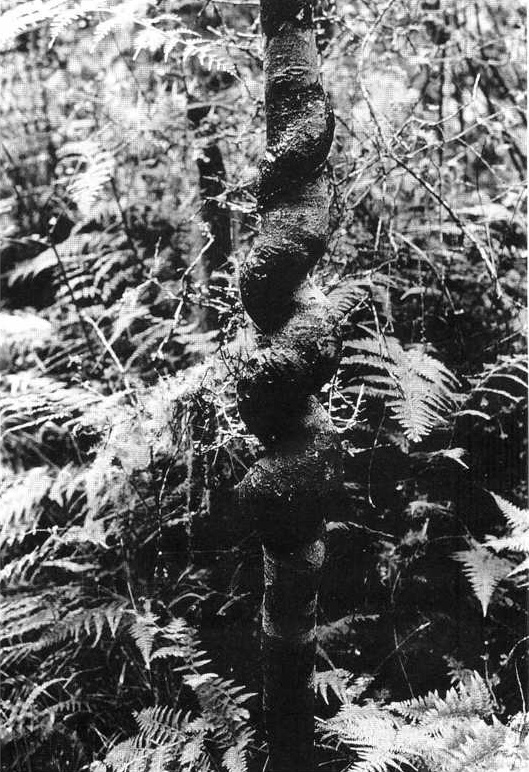
\includegraphics[width=0.66\textwidth]{graphics/figure35matai.jpg}
	\centering
	\caption[Stem of a young matai]{Stem of a young \IDX{matai} (\BotanicRef{Prumnopitys taxifalia}[Prumnopitys][taxifalia]) distorted by a twining vine (possibly \BotanicRef{Parsonsia heterophylla}[Parsonsia][heterophylla]) which subsequently died.
	Photo: J. W. Dawson.}%
	\label{fig:35matai}
\end{SCfigure}

By climbing up smaller trees \BotanicRef{Muehlenbeckia australis}[Muehlenbeckia][australis] may extend into the crowns of tall trees \SI{30}{\metre} or more above the ground.
A distinctive feature of \BotanicRef{Muehlenbeckia australis}[Muehlenbeckia][australis] is its formation of firm cane-like `searcher shoots' during the autumn from any part of the stem system.
Where these arise on stems coiled on the forest floor they grow erect for several metres, beginning to rotate only after the first metre.
Where they develop on stems in the tree crowns they extend more or less horizontally, often from one tree crown to another, and in this way the vines become extremely widespread through the forest canopy.
In fact, there sometimes seems to be more of the draping foliage of the \BotanicRef{Muehlenbeckia}, particularly in second growth forest, than of the trees themselves.
The adult leaves are several centimetres long; broad, thin and pale green, sometimes with a drawn-out tip.
Juvenile leaves are much smaller; round, oval or sometimes, fiddle-shaped.

\BotanicRef{Muehlenbeckia complexa}[Muehlenbeckia][complexa] is similar in its growth habit to \BotanicRef{Muehlenbeckia australis}[Muehlenbeckia][australis], but it is smaller in all respects and grows on shrubs or small trees at forest margins or in shrub associations.
The leaves are only about \SI{1}{\centi\metre} long, more or less circular and a little thicker than those of \BotanicRef{Muehlenbeckia australis}[Muehlenbeckia][australis].
The New Zealand species of the genus are largely endemic although \BotanicRef{Muehlenbeckia australis}[Muehlenbeckia][australis] occurs on Norfolk Island.
The genus also occurs in southern South America and Australia.

\BotanicRef{Tecomanthe speciosa}[Tecomanthe][speciosa] is undoubtedly New Zealand's rarest vine in nature, only one plant having been discovered, on the Three Kings Islands.
It has robust twining stems which, in cultivation, extend high into supporting trees.
The leaves are pinnately compound with quite large leathery leaflets and the tubular flowers, although large, are of an inconspicuous cream colour.
Most of the other species of \BotanicRef{Tecomanthe} are found in New Guinea.

Mangemange (\BotanicRef{Lygodium articulatum}[Lygodium][articulatum]) belongs to a largely tropical genus of ferns unique because of their ability to climb by twining; although in this case it is not the stems which twine but the axes of compound leaves, which have indefinite growth and sometimes extend from the ground to the tops of high trees.
The New Zealand species is restricted to the north of the North Island, but there it is common, particularly in \IDX{kauri forest}[kauri!forest]s.
The true stems spread over the forest floor.
The axes of the leaves arising from these are slender and wiry and often twine about each other as well as their supports to form springy masses on the ground, in well-lit places or on the forest roof.
Compound leaflets arise from the twining axes and, in well-lit situations, these may be fertile with narrow segments, each with two close-set rows of sporangia.

\subsection{Twining Leaf Petiole Climbers}

It might be wondered why the fern \BotanicRef{Lygodium}, with its twining leaves, is not included here.
Leaf climbers are defined as plants whose stems are supported as they grow upwards by the sensitive petioles (stalks) of their otherwise unmodified leaves, which wind round any slender supports with which they make contact.
In \BotanicRef{Lygodium} the true stems remain on the ground, but the primary axis of the leaf is like a twining stem in its indefinite growth and indefinite ability to twine.
Indeed it takes a botanist to appreciate that with \BotanicRef{Lygodium} we are dealing with twining leaves rather than twining stems, so it seems more realistic to treat it as a twiner rather than a leaf climber.

New Zealand representatives in this category are all species of \BotanicRef{Clematis}, a genus which is widespread in temperate regions and also found in the montane tropics.
The best known and largest New Zealand species is \BotanicRef{Clematis paniculata}[Clematis][paniculata], which is found in lowland forests throughout, particularly marginally, and is greatly appreciated in the spring when its sprays of large, pure-white flowers stand out against the dark foliage of the forest.
The adult leaves are divided into three leaflets, which are broad, dark-green, and smooth-margined.
Leaves on young plants on the forest floor are very different.
The first leaves are long, narrow, membranous in texture and undivided.
These are succeeded by compound leaves with three narrow leaflets.
In subsequent leaves, the leaflets become deeply lobed, broader, and, where light is adequate, gradually trend to the adult form.
Similar juvenile leaves have been reported for \BotanicRef{Clematis} species in eastern Australia.
Seedlings rotate in an anticlockwise direction and are able to twine around slender supports.
Similar twining ability, at least when young, has been recorded for some other leaf climbers outside New Zealand; nevertheless the primary mechanism for climbing is the clasping leaf petiole.

When a leaf is formed at a stem apex it is first erect, then gradually bends downward until it projects at right angles to the stem.
The petioles of the leaf as a whole, and of the leaflets, are well developed at this stage and if any of them touch a suitable support they are stimulated, by a process not yet understood, to wind round it.
The portion of the petiole in contact with the support enlarges and becomes strengthened.
Clearly the leaves cannot attach to large supports, so where a large stem of \BotanicRef{Clematis paniculata}[Clematis][paniculata] up to \SI{10}{\centi\metre} in diameter ascends to a tree crown \SI{10}{\metre} or more above the ground, it must have attained that position via smaller trees and shrubs.

The four or five other climbing New Zealand species of \BotanicRef{Clematis} are smaller than \BotanicRef{Clematis paniculata}[Clematis][paniculata].
They are incompletely known and in some cases not yet clearly defined.
Several grow at forest margins, including \BotanicRef{Clematis forsteri}[Clematis][forsteri] and \BotanicRef{Clematis foetida}[Clematis][foetida], and some also grow in shrubland.

\subsection{Tendril Climbers}

Tendrils are similar to the petioles of leaf climbers in that they are sensitive to touch and respond by twining round a support.
They differ in that they are derived from plant organs --- branches, inflorescences, leaves or leaflets --- which have completely lost their original function and are used solely for climbing.
Further, once a tendril has attached to a support, it coils into two opposed helices in its free part, which increases its elasticity and also draws the stem closer to the support.

In New Zealand we have only one forest liane which climbs by tendrils.
This is the native passion vine, \BotanicRef{Passiflora tetrandra}[Passiflora][tetrandra], which ranges through the North Island and down to Banks Peninsula on the east of the South Island.
The leaves are dark green and shiny and drawn out to a point at the tip.
The flowers are much smaller and less colourful than those of the cultivated species and less elaborate in their form, but the fruit compensates for this by being bright orange and \SIrange{2}{3}{\centi\metre} in diameter; it is greatly sought after by birds.

The tendrils arise in leaf axils and are considered to be modified inflorescences.
They are at first erect then bend downwards; if they encounter a slender support they wind round it.
The part in contact gradually becomes thickened, until it is about twice the diameter of the free part of the tendril.
The native passion vine is most common in the lower marginal parts of forests, but it spreads so effectively over the forest roof that it frequently reaches the tops of taller trees.
The woody stems can be up to \SI{12}{\centi\metre} in diameter and in their lower parts often form tortuous coils on the forest floor.

\subsection{Hook Climbers}

The New Zealand hook climbers are all species of \BotanicRef{Rubus}, a genus which includes the familiar blackberry and raspberry and is widespread in temperate regions and the montane tropics.
In north temperate regions, the species of \BotanicRef{Rubus} do not climb and are shrubs or scramblers in open habitats, but most of the New Zealand species and a number of Australian and tropical species are low to high climbing forest lianes.
The adult leaves of most species are palmately compound with three or more leaflets.
Backwardly curving hooks or prickles stud the underside of the petioles and leaflet midribs and sometimes the stem as well --- a feature which effectively prevents the stems slipping back from any position attained.
In colonial times, this tenacity earned for the New Zealand plant the name of `bush lawyer', a perhaps unwarranted slur on the legal profession of the day.
In fact the `lawyers' are the only plants in New Zealand forests which are prickly.
This is in contrast to the rain forests of Queensland and south-east Asia where many spiny climbers are unpleasantly in evidence.
The original lack of browsing mammals in New Zealand is the probable explanation for this, and the same would apply for the lack of spiny plants in New Caledonian forests.

The bush lawyers are sometimes included in the `scrambler' category of vines.
Scramblers are small, unspecialised climbers whose weak, drawn out stems grow up between the branches of shrubs and trail over them.
The lawyers begin their ascent in a similar way, but their hooks enable them to reach great heights, equal to those attained by more specialised vines.- For this reason I think they warrant a special category.
The liane species of New Zealand \BotanicRef{Rubus} occur throughout the country, including Fiordland, in lowland to montane forest.

\begin{SCfigure}[1.0][htb]
	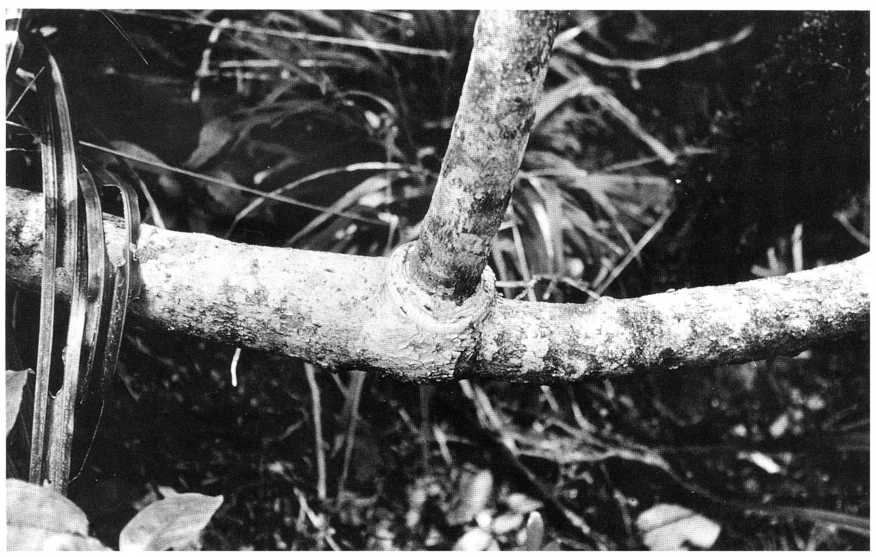
\includegraphics[width=0.66\textwidth]{graphics/figure36bushlawyer.jpg}
	\centering
	\caption[Bush lawyer]{Bush lawyer (\BotanicRef{Rubus cissoides}[Rubus][cissoides]).
	Horizontal stem near the ground with a vertical stem derived from a searcher shoot.
	Photo  J. W. Dawson.}%
	\label{fig:36bushlawyer}
\end{SCfigure}

The first leaves of the young plants are simple; their stems are quite stout and so are able to stand erect without support for \SI{60}{\centi\metre} or more.
If nothing is available to climb, the young plant bends to the ground, branches and spreads widely over the forest floor until some of the branches find supports and make their way into the forest canopy via shrubs and smaller trees.
The woody stems, which can be looped on the forest floor as well as extending to the forest roof, frequently produce `searcher shoots'\figureref{\fullref{fig:36bushlawyer}}.
The searcher shoots which are near to the ground can stand without support for one metre or more, and are thus very effective in expanding sites of \BotanicRef{Rubus} foliage in the canopy and in establishing new sites.

The commonest species is \BotanicRef{Rubus cissoides}[Rubus][cissoides] which has long, narrow and sharply toothed leaflets.
The adult stems may be up to \SI{17}{\centi\metre} in diameter and the foliage can reach to \SI{15}{\metre} or more above the ground.

\BotanicRef{Rubus schmidelioides}[Rubus][schmidelioides] has stems up to \SI{10}{\centi\metre} in diameter, and generally smaller, similarly shaped leaflets, but these leaflets are bluntly toothed and have a dense covering of whitish hairs beneath.

\BotanicRef{Rubus australis}[Rubus][australis] is most common in swamp forest and is sometimes referred to as `swamp lawyer'.
Its leaflets are short, fairly broad and sometimes almost circular.
In this species there is a distinct juvenile form, which spreads and roots widely over the forest floor, bearing leaves with small, membranous, more or less round leaflets with reddish coloured veins.
At the adult stage this species can reach for \SI{10}{\metre} or more into tree crowns, with stems several centimetres in diameter.

\BotanicRef{Rubus squarrosus}[Rubus][squarrosus] is perhaps the most remarkable of the genus, as, in open situations and on shrubs, the leaflet blades remain undeveloped and the leaves consist of rather elongated petioles and the almost threadlike midribs of the leaflets, all beset with yellow prickles\figureref{\fullref{fig:37rubus}}.
Such leaves are very effective in clinging to any support.
When the stems reach into tree crowns there is a trend towards normal leaves with well formed narrow leaflets.
This species is similar in eventual height and stem size to \BotanicRef{Rubus australis}[Rubus][australis].

\begin{SCfigure}[1.0][htb]
	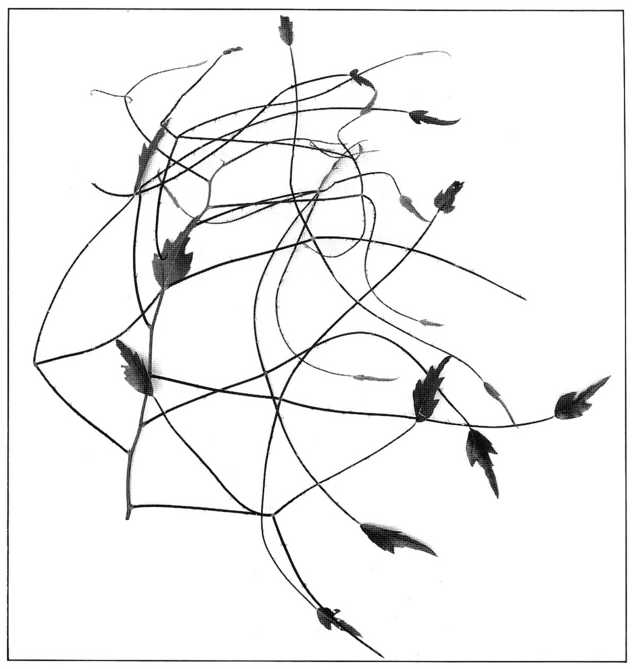
\includegraphics[width=0.5\textwidth]{graphics/figure37rubus.jpg}
	\centering
	\caption[\emph{Rubus squarrosus}]{\BotanicRef{Rubus squarrosus}[Rubus][squarrosus].
	Stems, leaf petioles and mostly bladeless leaflets beset with prickles.
	A few leaflet blades have developed.
	Photo: J. E. Casey.}%
	\label{fig:37rubus}
\end{SCfigure}

\section{Low Climbers of Forest Margins and Shrublands}

Some low climbers of more open habitats --- \BotanicRef{Parsonsia capsularis}[Parsonsia][capsularis], \BotanicRef{Muehlenbeckia complexa}[Muehlenbeckia][complexa], \BotanicRef{Clematis} (several species) --- have already been considered in association with their higher climbing relatives.

The remaining species are mostly unspecialised `scramblers', as defined in the last section in the discussion of hook climbers.
They grow through shrubs and small trees at forest margins or in shrub communities in drier eastern localities.
The species in this group are: \BotanicRef{Fuchsia perscandens}[Fuchsia][perscandens]; \BotanicRef{Brachyglottis sciadophilus}[Brachyglottis][sciadophilus] and \BotanicRef{Helichrysum dimorphum}[Helichrysum][dimorphum] of the Compositae or daisy family; \BotanicRef{Scandia geniculata}[Scandia][geniculata] of the Umbelliferae or carrot family (perhaps the only climbing member of this family); \BotanicRef{Carmichaelia kirkii}[Carmichaelia][kirkii], one of the leafless brooms; and an undescribed species of \BotanicRef{Coprosma}.\footnote{\cite{eagle1982trees}}

One of our species of \BotanicRef{Lycopodium}, the attractive trailing \BotanicRef{Lycopodium volubile}[Lycopodium][volubile], can also be a scrambling climber over shrubs.
This species ranges from New Zealand to the tropical Pacific and south east Asia and, in the latter region, is recorded as sometimes extending into tree crowns.

\section{Vines Growing as Shrubs in Open Situations}

A number of vines can grow as shrubs in open situations where there is no support.
This is particularly the case with the small, unspecialised, scrambling species, as well as the small twiners \BotanicRef{Muehlenbeckia complexa}[Muehlenbeckia][complexa] and \BotanicRef{Parsonsia capsularis}[Parsonsia][capsularis], both of which are able to make an easy transition from well lit forest margin and shrubby habitats to completely open sites.
As shrubs these species often have a ball-like form with a profusion of slender, entangled stems.

Some of the taller, more specialised forest vines may also grow as shrubs. \BotanicRef{Rubus squarrosus}[Rubus][squarrosus] has been already mentioned.
Several of the climbing \IDX{rata}s (\BotanicRef{Metrosideros}) can also be encountered as shrubs. \BotanicRef{Metrosideros perforata}[Metrosideros][perforata] in particular has a dense, billowy form, which gives no hint of any ability to climb.
Such dual roles are not peculiar to New Zealand vines, but have also been observed in a number of tropical lianes.\footnote{\cite{richards1952tropical}}

\section{Epiphytes}

Sharing a need for much brighter light than is available on the floor of a closed forest, the majority of species of epiphytes, vines and parasites grow high in tree crowns.
In this situation epiphytes alone face special problems.
Vines are able to obtain soil, water and mineral nutrients via their stems; parasites can tap the supplies drawn up by their host trees; but epiphytes either have no connection with the ground throughout their lives or send roots down to it only after a period of some years.
Soil does not form easily on trunks and branches and as they are sunnier, windier and better drained than the ground, they suffer both more frequent and more severe droughts.
In response to these stressful conditions, many epiphytes have evolved modifications enabling them to store water and to reduce its loss by evaporation as well as to build up a layer of water-retentive soil.
Water can be stored internally in special cells, whose presence confers fleshiness on the organs concerned, or externally in cavities formed by appropriately shaped and arranged leaves.
Some epiphytes can get by with a minimum of mineral nutrients and need little or no soil; others build up considerable quantities of dark humus, largely from the decay of their own old leaves and roots with a varying contribution of bark flakes and leaves from surrounding trees.
Many other epiphytes which are unable to form soil themselves take advantage of those that can.

Now we have defined the epiphyte category, how rigorously do we interpret the definition in deciding whether or not a particular species should be included? Certainly not so rigorously that we exclude those species which, although normally epiphytic, are sometimes to be found on sunny, rock outcrops which provide conditions similar to those of tree tops.
In fact, it might well be that there are no epiphytes, even those of tropical forests, unable to grow on the ground in suitable circumstances.

Going to the other extreme, should we include species which are normally terrestrial, but can occasionally grow on trees? In this case the answer is `no' as, apart from reservations about stretching the definition so far, the number of species involved would be inconveniently large.
In certain circumstances almost any plant is able to grow as an epiphyte.
For example, in forests of high rainfall, particularly where frequent mists maintain high atmospheric humidity, seeds germinate just as readily on moist, moss and lichen covered trunks and branches as on the ground.
A notable example of chance epiphytism in these circumstances in New Zealand is an occasional \IDX{silver beech}[beech!silver] (\BotanicRef{Nothofagus menziesii}[Nothofagus][menziesii]) growing on a tree of the same species.
Even in forests of average rainfall and atmospheric humidity, the branch systems of large, long-lived trees, such as the \IDX{kauri}, are available as habitats for so many centuries that quite unlikely species can sometimes be found as epiphytes on them.
The intrepid Harrison-Smith\footnote{\cite{harrisonsmith1938kauri}} found a \SI{3}{\metre} \IDX{kauri} growing on a \IDX{kauri}, as well as several examples of other conifers --- \IDX{rimu}, \IDX{totara}, \IDX{kahikatea} and several angiosperm trees.
In most cases the occasional epiphytic plants of otherwise terrestrial trees and shrubs are small and do not grow to reproductive maturity.

Lichens, often followed by mosses, are generally the first epiphytes on trees in both temperate and tropical regions.
In New Zealand small filmy ferns are frequently associated with the mosses.
The thin layer of soil that these small epiphytes form is important for the establishment of most of the vascular epiphytes,\footnote{\cite{oliver1930new}} which are the concern of this section.

\section{Shade Epiphytes}

These do not require a very high level of light, and as epiphytes they mostly grow low on tree trunks where they escape the shading of the larger plants of the forest floor.

Six small species of fern and two flowering plants occupy this station in New Zealand, although they may also be found on rocks.
Of the ferns, three are species of \BotanicRef{Grammitis} characterised by tufts of narrow simple leaves arising from short rhizomes. \BotanicRef{Grammitis pseudociliata}[Grammitis][pseudociliata] differs from \BotanicRef{Grammitis billardieri}[Grammitis][billardieri] and \BotanicRef{Grammitis magellanica subsp.\ nothofageti}[Grammitis][magellanica subsp.\ nothofageti] in having an abundance of reddish hairs on its leaves. \BotanicRef{Grammitis pseudociliata}[Grammitis][pseudociliata] is concentrated in the North Island; \BotanicRef{Grammitis billardieri}[Grammitis][billardieri] and \BotanicRef{Grammitis magellanica}[Grammitis][magellanica] extend throughout the country, the last also occurring in south-east Australia.

\BotanicRef{Ctenopteris heterophylla}[Ctenopteris][heterophylla] occurs throughout the country as well as in the subantarctic islands and south-east Australia.
Its habit is similar to that of the \BotanicRef{Grammitis} species, but the leaves are somewhat larger and oncepinnate with toothed leaflets.

\BotanicRef{Anarthropteris lanceolata}[Anarthropteris][lanceolata] is found in the North Island and near the northern shores of the South Island, as an epiphyte or on rocks.
It is also said to occur in Vanuatu.
The leaves are very similar in shape to those of \BotanicRef{Grammitis} but longer.
The rhizomes are short and produce masses of slender furry roots, some of which can give rise to new tufts of leaves.

These five epiphytic ferns are related to the climbing \BotanicRef{Phymatosorus} species and have similar prominent, rounded to oblong, brown to orange sori.
The sixth fern which grows as a low epiphyte is a filmy fern, \BotanicRef{Hymenophyllum pulcherrimum}[Hymenophyllum][pulcherrimum], which ranges throughout the country.

The two flowering low epiphytes are both species of \BotanicRef{Peperomia}, a large genus of small succulent plants in tropical and subtropical regions.
As epiphytes, they grow mostly near the coast in the northern half of the North Island. \BotanicRef{Peperomia tetraphylla}[Peperomia][tetraphylla] ranges from the East Cape district through to the Bay of Plenty.
It has leaves in whorls of four as its name indicates.
The same species is also found in Australia and Polynesia, \BotanicRef{Peperomia urvilleana}[Peperomia][urvilleana] bears its leaves singly and grows throughout the North Island and near the northern shores of the South Island, but is less common in the southern part of its range and there grows mostly on rocks.
It is found also on Norfolk and Lord Howe Islands.

\section{Sun Epiphytes}

These are most abundant in tree crowns, although some also occur at lower, shadier levels.
Sun epiphytes are more numerous and diverse than shade epiphytes and can be grouped into several growth forms.

\subsection{Mat Epiphytes}

\begin{SCfigure}[1.0][htb]
	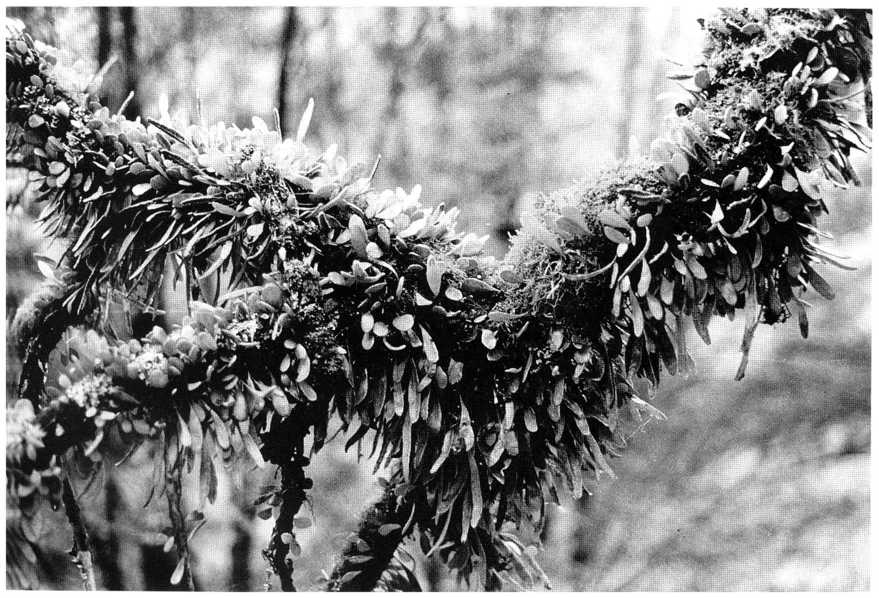
\includegraphics[width=0.66\textwidth]{graphics/figure38pyrrosia.jpg}
	\centering
	\caption[\emph{Pyrrosia serpens}, a fern mat epiphyte]{\BotanicRef{Pyrrosia serpens}[Pyrrosia][serpens], a fern mat epiphyte.
	Photo  J. W. Dawson.}%
	\label{fig:38pyrrosia}
\end{SCfigure}

These epiphytes form mats or patches mostly on inclined or horizontal branches, and they comprise three orchids and one fern which range throughout the country.
Mat epiphytes may establish directly on bare bark, particularly if it is rough and fissured, but may also avail themselves of moss cushions.
The fern is \BotanicRef{Pyrrosia serpens}[Pyrrosia][serpens]\figureref{\fullref{fig:38pyrrosia}}, which belongs to a genus of epiphytes centred in tropical Asia.
Our species is also found in Australia and the islands of Polynesia. \BotanicRef{Pyrrosia} often establishes directly on bare bark and has slender, freely branching rhizomes which form a complete network over sunny branches.
The leaves are simple and smooth-margined, varying from almost round to long and narrow.
They have a fleshy texture and a dense felt of buff coloured hairs beneath, which presumably restrict loss of water. \BotanicRef{Pyrrosia} also grows on the trunks of trees in the open and on rocks.
It can be quite abundant on introduced trees, particularly \BotanicRef{Cupressus macrocarpa}[Cupressus][macrocarpa].

The epiphytic orchids\footnote{\cite{hatch1948epiphytic}} which form mats or patches belong, or are closely related, to large tropical genera and can be regarded as outliers, reduced in both leaf and flower size.
They all have specialised roots which, as well as serving for attachment, also efficiently absorb and store water in a special outer layer of dead cells known as the velamen.

\BotanicRef{Drymoanthus adversus}[Drymoanthus][adversus], often attached to quite smooth bark, is unlike the other species in that it has a short stem, which does not grow along the bark surface.
The roots arising at the base of the tuft of leaves are particularly conspicuous as they spread out `like the rays of a spider's web' for a considerable distance, often encountering the roots of other plants of the same species. \BotanicRef{Drymoanthus} includes our species, another in east Australia and a third in \IDX{New Caledonia}, but there is some doubt as to whether it should be separated from the Asian and Australian genus \BotanicRef{Sarcochilus}.
Our two species of \BotanicRef{Bulbophyllum}, although small, form quite dense patches with their branching rhizomes.
In common with their many tropical relatives, each of their rhizome segments swells at the end into a water-storing `pseudobulb' with a single leaf arising from the top.
The stalk bearing the small flower or flowers arises from below the pseudobulb. \BotanicRef{Bulbophyllum pygmaeum}[Bulbophyllum][pygmaeum] is the smaller species with leaves about a centimetre long but it forms larger patches than those of \BotanicRef{Bulbophyllum tuberculatum}[Bulbophyllum][tuberculatum].
The leaves of \BotanicRef{Bulbophyllum tuberculatum}[Bulbophyllum][tuberculatum] are several times longer, but this species is less frequently seen and is not known further south than the north coast of the South Island.

\subsection{Nest Epiphytes}

\begin{figure}[!htb]
	% Outer minipage scaled to limit width.
	% Inner minipages scaled so the images have the same height.
	\begin{minipage}[t]{\textwidth}
		\begin{minipage}[t]{(\textwidth-\fgap) * \real{0.446}}
			\centering
			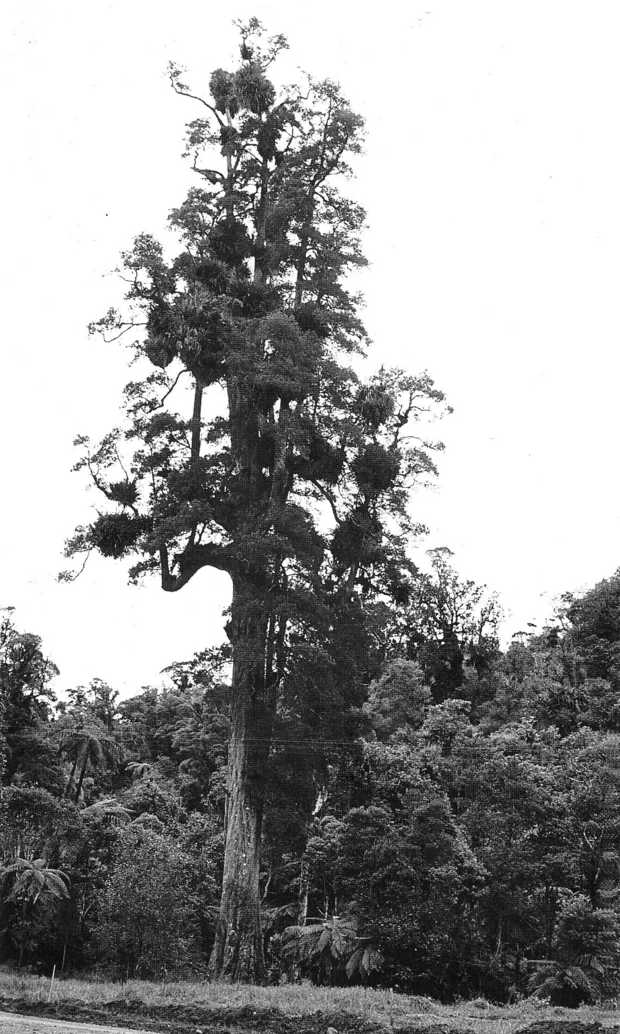
\includegraphics[width=\textwidth]{graphics/figure39kahikatea.jpg}
			\caption[Tall kahikatea with many asteliad nests]{Tall \IDX{kahikatea} (\BotanicRef{Dacrycarpus dacrydioides}[Dacrycarpus][dacrydioides]) with many asteliad nests.
			South of Kaitaia, northern North Island.
			Photo: B. V. Sneddon.}%
			\label{fig:39kahikatea}
		\end{minipage}\hspace{\fgap}%
		\begin{minipage}[t]{(\textwidth-\fgap) * \real{0.554}}
			\centering
			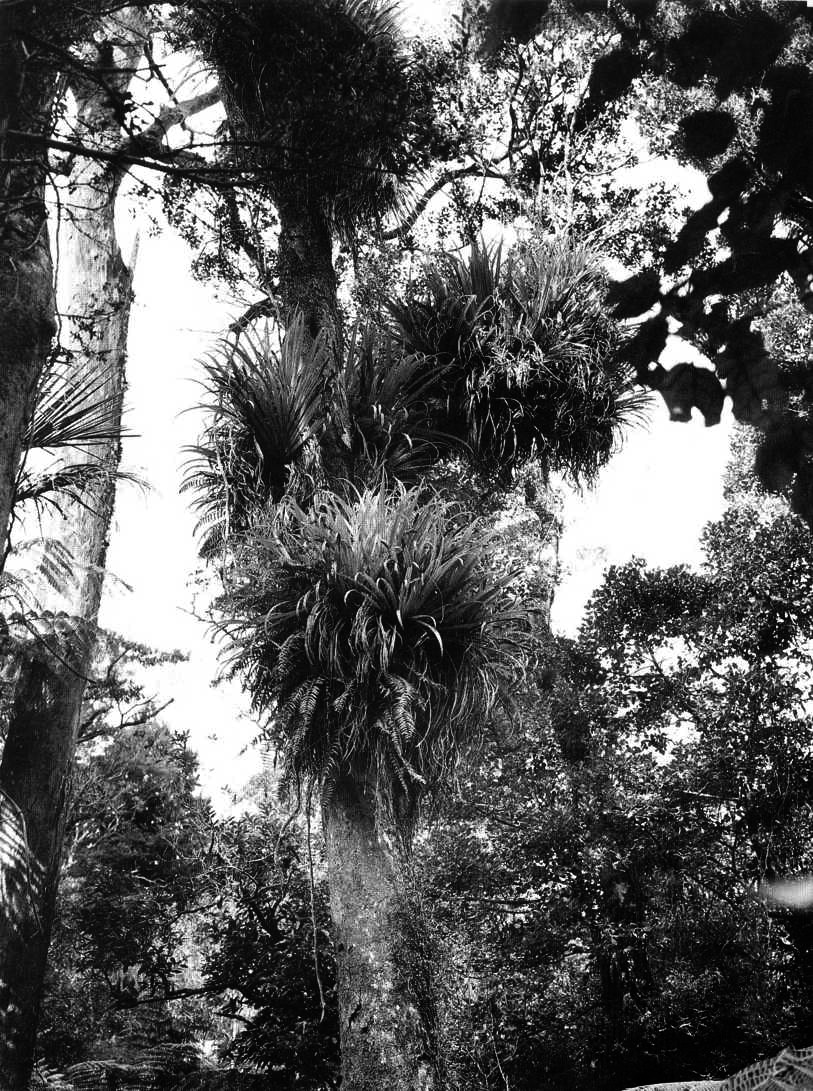
\includegraphics[width=\textwidth]{graphics/figure40asteliad.jpg}
			\caption[Asteliad nests with the pendent epiphytic fern]{Asteliad nests with the pendent epiphytic fern \BotanicRef{Asplenium polyodon}[Asplenium][polyodon] below them.
			Photo: M. D. King.}%
			\label{fig:40asteliad}
		\end{minipage}
	\end{minipage}
\end{figure}

Much more evident to the casual observer are the massive nest epiphytes perched high in tree crowns\figureref{\fullref{fig:26kahikatea}, \fullref{fig:39kahikatea}, \fullref{fig:40asteliad}}.
In New Zealand there are three long and narrow-leaved species belonging to two closely related genera of the lily family --- \BotanicRef{Collospermum hastatum}[Collospermum][hastatum], \BotanicRef{Collospermum microspermum}[Collospermum][microspermum] and \BotanicRef{Astelia solandri}[Astelia][solandri].
Two other species of \BotanicRef{Collospermum} are found outside New Zealand, one each in Fiji and Samoa; both are epiphytes.
In the much larger and more widespread \BotanicRef{Astelia} found mostly in the southern hemisphere, only a few species are consistently epiphytic.
The others are found in New Zealand in a variety of habitats --- coastal cliffs, swamps, forest floors, alpine tussock grassland and a few reduced turf-forming species in alpine bogs.

All three nest epiphytes usually establish among mosses and lichens in branch forks or on inclined or horizontal branches.
As their stems, completely hidden by the leaf clusters, are short and more or less erect the plants are fixed in position; although when they branch to form additional leaf clusters the resulting massive clumps of foliage may be metres in diameter.
The `nests' are attached to their supports by extensive root systems and as the old roots and leaves die and decay, considerable depths of dark spongy soil are built up.
The likely eventual fate of these large soil and plant masses is to fall to the ground.
Heavy rain absorbed by the soil greatly increases the weight of the mass and if the rain is accompanied by wind, complete branches may crash to the ground under the weight of epiphytes.

\BotanicRef{Astelia solandri}[Astelia][solandri] is more shade tolerant than the collospermums and so is often found below them in the lower crowns and on the upper trunks of trees.
The silvery green leaves are in three ranks and are \SIrange{1}{2}{\metre} long, but only \SIrange{2}{3}{\centi\metre} wide.
Their bases are tightly folded, forming a narrow ridge at the back. \BotanicRef{Astelia solandri}[Astelia][solandri] is found in lowland forests throughout the North Island, near the northern coast and down the western side of the South Island to about \ang{44} S.

\begin{SCfigure}[2][htb]
	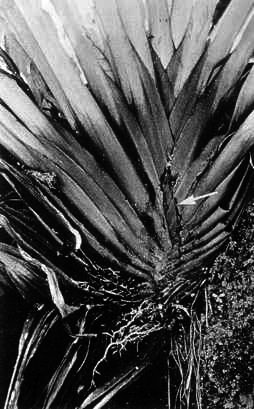
\includegraphics[width=0.33\textwidth]{graphics/figure41collospermum.jpg}
	\centering
	\caption[Close view of a Collospermum hastatum leaf fan]{Close view of a \BotanicRef{Collospermum hastatum}[Collospermum][hastatum] leaf fan showing the dark leaf bases and roots between the decaying outer leaves.
	The arrow indicates where water is seeping from the reservoirs between the leaves.
	Photo: J. W. Dawson.}%
	\label{fig:41collospermum}
\end{SCfigure}

\BotanicRef{Collospermum hastatum}[Collospermum][hastatum] accompanies \BotanicRef{Astelia solandri}[Astelia][solandri] through the North Island and to about \ang{42;30;} in the South Island. \BotanicRef{Collospermum microspermum}[Collospermum][microspermum] is restricted to the North Island and replaces \BotanicRef{Collospermum hastatum}[Collospermum][hastatum] in montane forests above about 300 m. \BotanicRef{Collospermum hastatum}[Collospermum][hastatum] has fan-like arrangements of black-based leaves\figureref{\fullref{fig:41collospermum}} which are somewhat shorter and much broader than those of \BotanicRef{Astelia solandri}[Astelia][solandri].
The bases of the leaves are strongly rounded and enclose spaces or `tanks' which become filled with water when it rains.
Often sufficient water is contained by the tanks to provide a shower bath for the unwary when a fallen \BotanicRef{Collospermum} nest is lifted and tilted.
A species of mosquito has been described whose larvae always develop in the water stored by \BotanicRef{Collospermum hastatum}[Collospermum][hastatum]\footnote{\cite{belkin1968mosquito}} but this is a very modest fauna compared with the many insects and even frogs which inhabit the `tanks' of the tropical American epiphytes of the Bromeliaceae (pineapple family).
The water stored by \BotanicRef{Collospermum hastatum}[Collospermum][hastatum] is partly absorbed by roots which grow into the tanks, but the suggestion that it is also absorbed through the embedded multicellular bases of overlapping scales has not been confirmed.
In some tropical bromeliads all of the stored water is absorbed through the bases of similar scales.

\BotanicRef{Collospermum microspermum}[Collospermum][microspermum] is equally specialised but its leaves are as narrow as those of \BotanicRef{Astelia solandri}[Astelia][solandri] and dark-brown rather than black at the base.

The collospermums are the only known tank epiphytes outside the family Bromeliaceae, but as they form soil very efficiently, they are also nest epiphytes.

\subsection{Pendent Epiphytes}

\begin{figure}[!htb]
	% Outer minipage scaled to limit width.
	% Inner minipages scaled so the images have the same height.
	\begin{minipage}[t]{0.7\textwidth}
		\begin{minipage}[t]{(\textwidth-\fgap) * \real{0.564}}
			\centering
			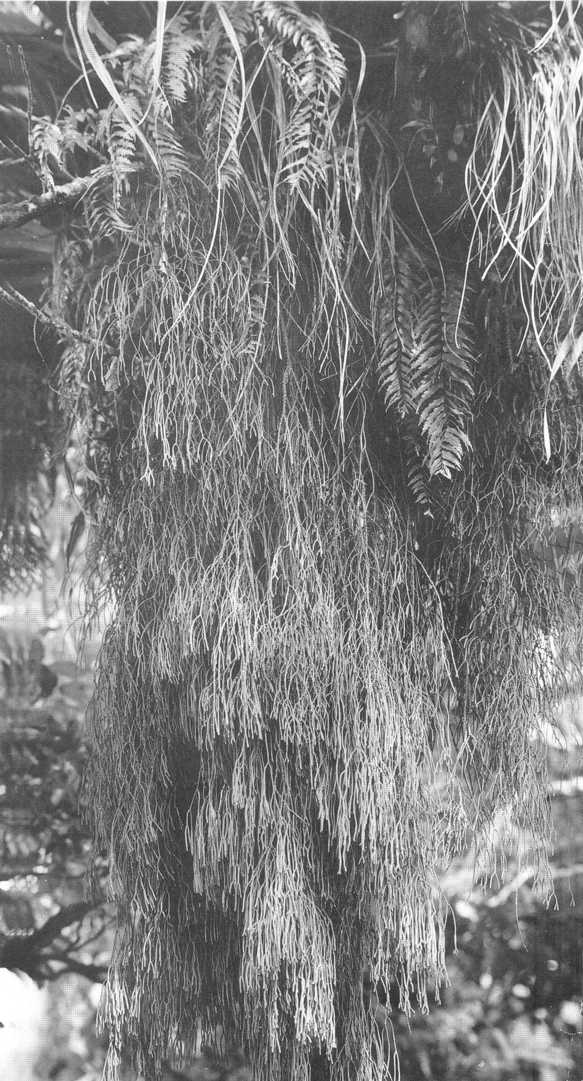
\includegraphics[width=\textwidth]{graphics/figure42lycopodium.jpg}
			\caption[Hanging tassels of Lycopodium varium]{Hanging tassels of \BotanicRef{Lycopodium varium}[Lycopodium][varium] below an asteliad nest.
			Photo: M. D. King.}%
			\label{fig:42lycopodium}
		\end{minipage}\hspace{\fgap}%
		\begin{minipage}[t]{(\textwidth-\fgap) * \real{0.436}}
			\centering
			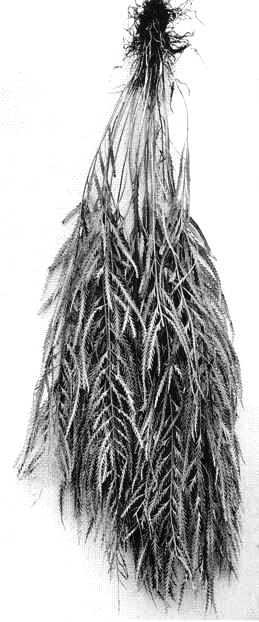
\includegraphics[width=\textwidth]{graphics/figure43asplenium-jlaccidum.jpg}
			\caption[Epiphytic plant of the fern \emph{Asplenium flaccidum}]{Epiphytic plant of the fern \BotanicRef{Asplenium flaccidum}[Asplenium][flaccidum].
			Photo: M. D. King.}%
			\label{fig:43asplenium-jlaccidum}
		\end{minipage}
	\end{minipage}
\end{figure}

Four New Zealand wide pteridophyte species often grow as epiphytes with their roots or rhizomes embedded in the soil of epiphyte nests.
Though they occur elsewhere as well it is in these sites that their growth is most vigorous and their pendulous stems or leaves attain their maximum length.
Of the four, \BotanicRef{Lycopodium varium}[Lycopodium][varium] is the most impressive; its slender stems sometimes forming huge masses up to \SI{1.5}{\metre} long, below asteliad nests\figureref{\fullref{fig:42lycopodium}}.
The stems branch repeatedly by equal forkings or dichotomies, so that they form a dense but well balanced mass.
It is almost constantly in motion as even the lightest breeze can set the tassels swaying.
In their upper parts the stems are clothed by small spreading leaves, which grade into small, close-set scales enclosing the sporangia towards the branch tips. \BotanicRef{Lycopodium varium}[Lycopodium][varium] is restricted to New Zealand, but there are related species in tropical forests.

The ferns \BotanicRef{Asplenium polyodon}[Asplenium][polyodon] (= \BotanicRef{Asplenium falcatum}[Asplenium][falcatum]) and \BotanicRef{Asplenium flaccidum}[Asplenium][flaccidum] may have leaves of a metre or more in length below the epiphyte nests. \BotanicRef{Asplenium polyodon}[Asplenium][polyodon], with its double-toothed, wedge-shaped leaflets is perhaps the most attractive of the New Zealand species of the genus\figureref{\fullref{fig:40asteliad}}. \BotanicRef{Asplenium flaccidum}[Asplenium][flaccidum] has an unusual stringlike appearance with long and narrow, deeply-toothed leaflets\figureref{\fullref{fig:43asplenium-jlaccidum}}.
Dobbie aptly describes the leaves of this species as appearing to have been `cut from a piece of pale-green leather'. \BotanicRef{Asplenium polyodon}[Asplenium][polyodon] is found from India to Australia and the Pacific and \BotanicRef{Asplenium flaccidum}[Asplenium][flaccidum] in Australia and some Pacific Islands.
Both Aspleniums and \BotanicRef{Lycopodium varium}[Lycopodium][varium] extend into montane cloud forests, but there they depend from mossy trunks and branches.

\BotanicRef{Tmesipteris}, a genus restricted to the south west Pacific, is sometimes referred to as a `living fossil' as it is considered to be one of the most primitive genera of land plants.
One of the highlights for botanical visitors to New Zealand is to see a living plant of this genus. \BotanicRef{Tmesipteris elongata subsp.\ robusta}[Tmesipteris][elongata subsp.\ robusta] has been observed growing from \BotanicRef{Collospermum} clumps at a number of localities through the North Island, but not yet in the South Island.
Its stems, with their small, simple leaves, are unusually long for a \BotanicRef{Tmesipteris} and dichotomise freely.
Other species of \BotanicRef{Tmesipteris} rarely branch.

Three orchid species can also be included as pendent epiphytes.
The two Earinas belong to a small genus with other species in \IDX{New Caledonia} and Polynesia, but this genus is considered to be closely related to the larger \BotanicRef{Epidendrum} of tropical America.
Both species have spreading rhizomes and can sometimes extend for several metres along branches.
The stems bearing the leaves droop downwards and can be \SI{30}{\centi\metre} or more long.
The leaves are formed in two rows, more or less in one plane; those of \BotanicRef{Epidendrum mucronata}[Epidendrum][mucronata] are narrow, thin and quite grasslike while those of \BotanicRef{Epidendrum autumnalis}[Epidendrum][autumnalis] are broader and thicker, in keeping with the more robust nature of the plant as a whole.
Both species form terminal sprays of small flowers, \BotanicRef{Epidendrum mucronata}[Epidendrum][mucronata] in the spring and \BotanicRef{Epidendrum autumnalis}[Epidendrum][autumnalis] in the autumn.
The flower clusters of \BotanicRef{Epidendrum mucronata}[Epidendrum][mucronata] hang down and are yellowish orange, those of \BotanicRef{Epidendrum autumnalis}[Epidendrum][autumnalis] turn upwards and are waxy white with a strong spicy perfume.

Our sole species of the large tropical genus \BotanicRef{Dendrobium} (\BotanicRef{Dendrobium cunninghamii}[Dendrobium][cunninghamii]) is the largest of New Zealand's epiphytic orchids.
Its freely branching stems and narrow leaves form feathery drooping masses.
The stems are polished, often bright yellow and very bamboo-like in appearance.
The white, reddish-centred flowers are scattered and while modest by tropical standards are, at \SIrange{2}{2.5}{\centi\metre} in diameter, the largest among our epiphytic orchids.

\subsection{Small Shrub Epiphytes}

The two species of \BotanicRef{Pittosporum} and one each of \BotanicRef{Senecio} and \BotanicRef{Coprosma} in this category are not usually more than a metre high when growing as epiphytes, but may attain small tree size on the ground.
All are endemic to New Zealand.

\BotanicRef{Pittosporum cornifolium}[Pittosporum][cornifolium] is found throughout the North Island and although it is quite a common plant, many people are unaware of its existence, perched as it is inconspicuously in tree crowns.
The stems of this plant are spindly and often hang down below the branches.
The leaves are thin but firm with prominent veins and the flowers are small and yellowish red.
The round, woody seed capsules are a surprise.
When they open they reveal a bright red lining and shiny black seeds embedded in sticky, bright yellow fluid.

\BotanicRef{Pittosporum kirkii}[Pittosporum][kirkii] has a more restricted range, as it is not found further south than the central North Island.
It has a more erect growth habit with thicker stems and longer, thicker, almost fleshy leaves with obscure veins.
The flowers are bright yellow and the capsules are unusually large (up to \SI{4}{\centi\metre} long), flattened and pod-like.
Kirk,\footnote{\cite{kirk1869botany}} after whom the species is named, states that the `valves contract in a curious manner when the capsule bursts'.
The capsule is apparently not so colourful as that of \BotanicRef{Pittosporum cornifolium}[Pittosporum][cornifolium], but is described as having an orange lining.

\BotanicRef{Brachyglottis kirkii}[Brachyglottis][kirkii] is found in lowland forests throughout the North Island but has not been recorded from the South Island.
Its growth form has been described as `candelabra-like'\figureref{\fullref{fig:44brachyglottis-kirkii}}.
The leaves are soft and somewhat fleshy and the flowers, up to \SI{5}{\centi\metre} in diameter, pure white and crowded into dense heads.

The thick and shiny-leaved karamu (\BotanicRef{Coprosma lucida}[Coprosma][lucida]) is best known as a ground plant in shrubby, early forest regrowth on drier sites, but is also reasonably common as an epiphyte in asteliad nests.
The species is found throughout the country but presumably is common as an epiphyte only within the range of nest epiphytes.

\begin{figure}[htb]
	% Outer minipage scaled to limit width.
	% Inner minipages scaled so the images have the same height.
	\begin{minipage}[t]{\textwidth}
		\begin{minipage}[t]{(\textwidth-\fgap) * \real{0.497}}
			\centering
			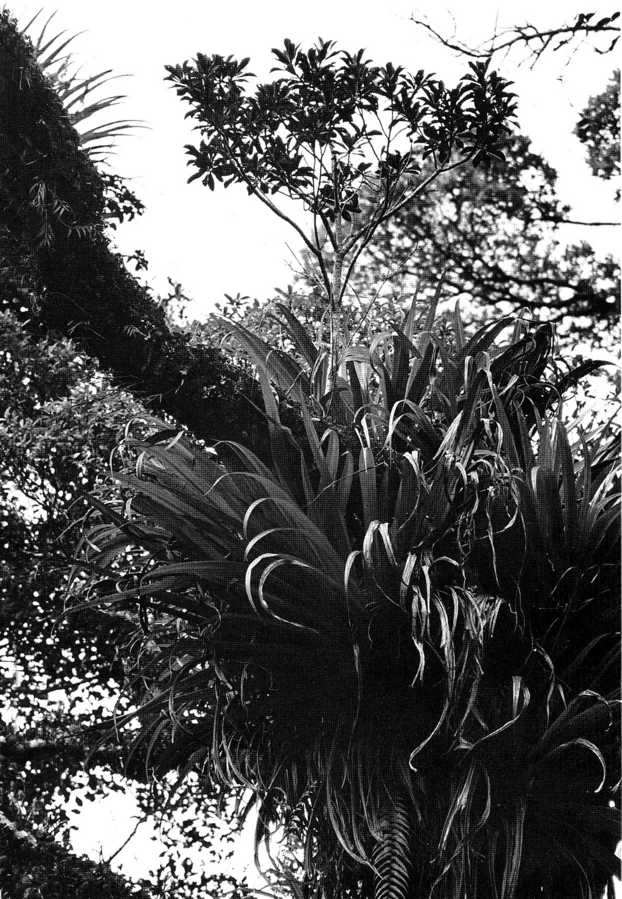
\includegraphics[width=\textwidth]{graphics/figure44brachyglottis-kirkii.jpg}
			\caption[The small epiphytic shrub \emph{Brachyglottis kirkii}]{The small epiphytic shrub \BotanicRef{Brachyglottis kirkii}[Brachyglottis][kirkii] growing from an asteliad nest.
			Photo: B. V. Sneddon.}%
			\label{fig:44brachyglottis-kirkii}
		\end{minipage}\hspace{\fgap}%
		\begin{minipage}[t]{(\textwidth-\fgap) * \real{0.503}}
			\centering
			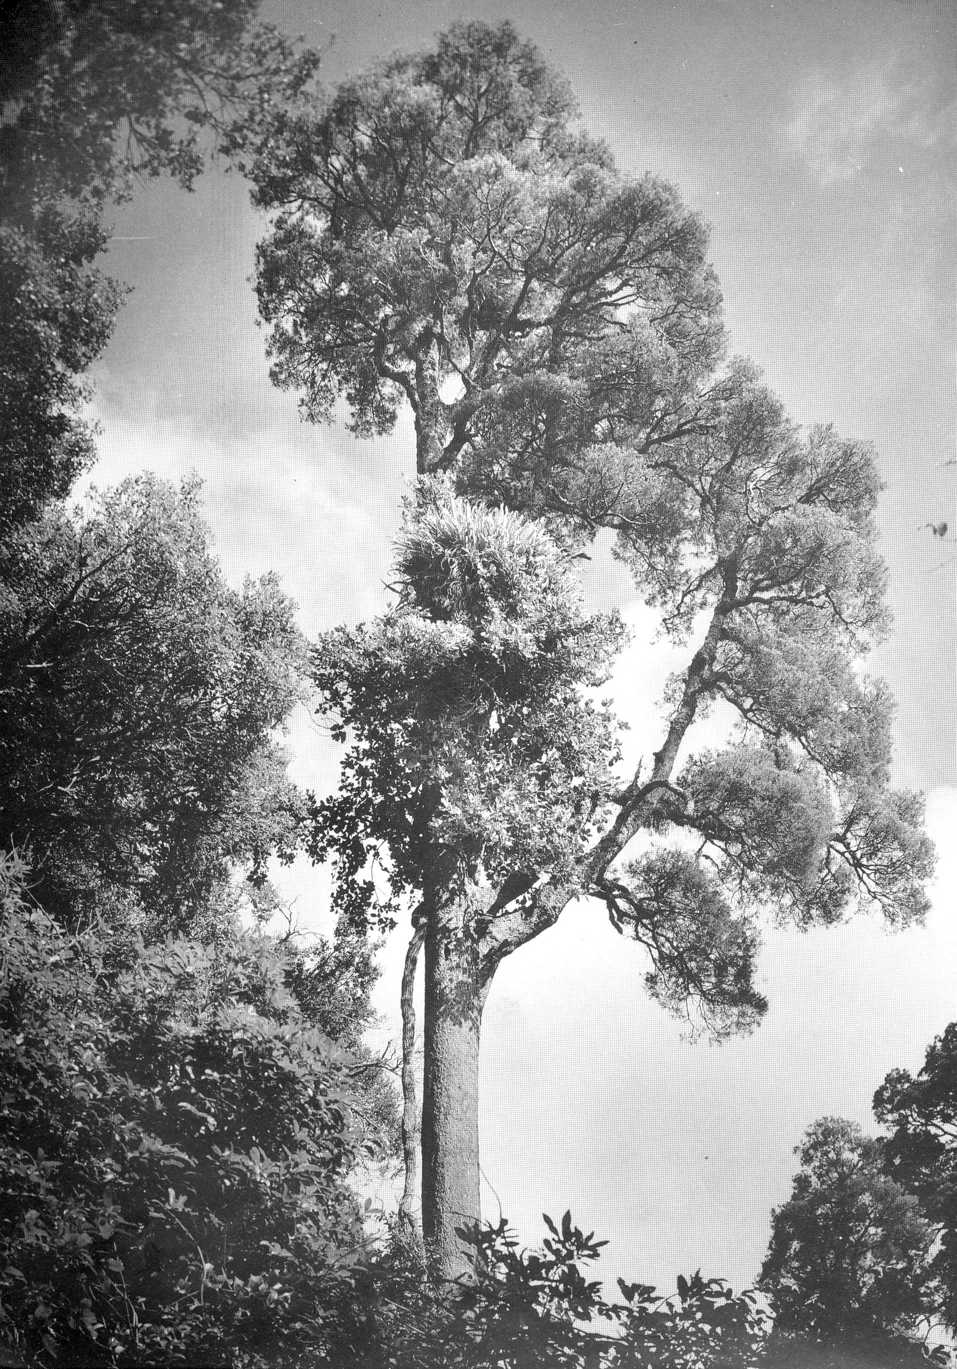
\includegraphics[width=\textwidth]{graphics/figure45puka.jpg}
			\caption[The large shrub epiphyte puka]{The large shrub epiphyte \IDX{puka} (\BotanicRef{Griselinia lucida}[Griselinia][lucida]) on a \IDX{kahikatea}.
			The crown of the \IDX{puka} is just below an asteliad nest and its main descending root is to the left of the tree trunk.
			Te Marua, southern North Island.
			Photo: M. D. King.}%
			\label{fig:45puka}
		\end{minipage}
	\end{minipage}
\end{figure}

\subsection{Large Shrub Epiphytes}

As well as being larger than those of the preceding category, these also eventually send a root to the ground and so overcome the water supply and soil nutrient problem.

\IDX{Puka}[puka] (\BotanicRef{Griselinia lucida}[Griselinia][lucida])\footnote{\cite{dawson1966vegetative}} is the most notable in this category.
Its large, dark green shining leaves usually contrast so strongly with the foliage of the supporting tree that it stands out even to the casual observer\figureref{\fullref{fig:45puka}}.
\IDX{Puka}[puka] is distributed in lowland forests throughout the North and South Islands, but is more common in the north.
Its seedlings generally establish in asteliad nests situated at branch forks and its roots ramify through the humic soil.
After a few years a strong root begins to grow down the trunk of the supporting tree towards the ground.
This root and its branches are closely appressed to the bark of the trunk, and frequently grow into crevices and behind bark flakes.
The root tips are white and smooth, but a short distance away from them the root surfaces are often densely clothed with short root hairs.
Where the roots are in contact with the trunk, they are anchored by the root hairs and the union is sometimes so complete that when the roots are pulled away they either remove portions of bark or leave strips of their own tissue behind.

\begin{figure}[htb]
	% Outer minipage scaled to limit width.
	% Inner minipages scaled so the images have the same height.
	\begin{minipage}[t]{\textwidth}
		\begin{minipage}[t]{(\textwidth-\fgap) * \real{0.495}}
			\centering
			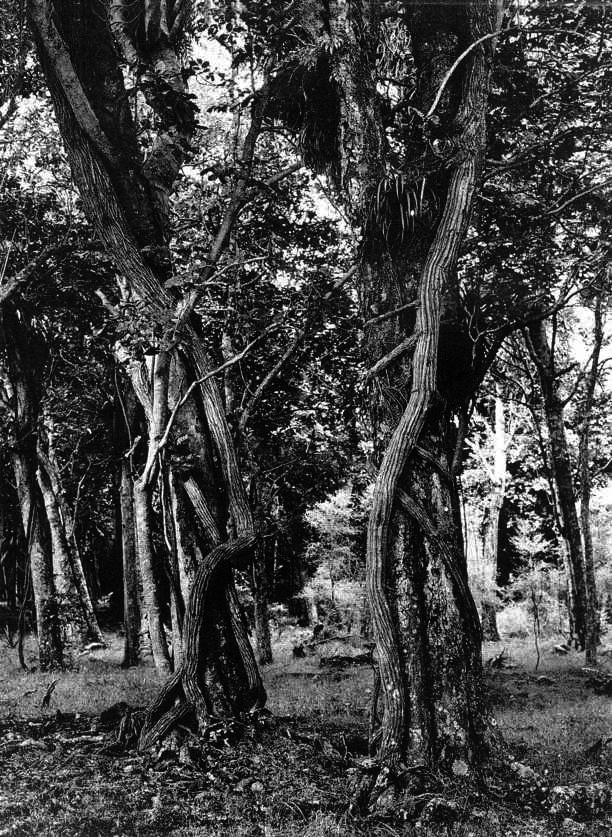
\includegraphics[width=\textwidth]{graphics/figure46puka-roots.jpg}
			\caption[Distinctively fluted roots of puka on kohekohes]{Distinctively fluted roots of \IDX{puka} (\BotanicRef{Griselinia lucida}[Griselinia][lucida]) on \IDX{kohekohe}s.
			Waikanae, southern North Island.
			Photo: M. D. King.}%
			\label{fig:46puka-roots}
		\end{minipage}\hspace{\fgap}%
		\begin{minipage}[t]{(\textwidth-\fgap) * \real{0.505}}
			\centering
			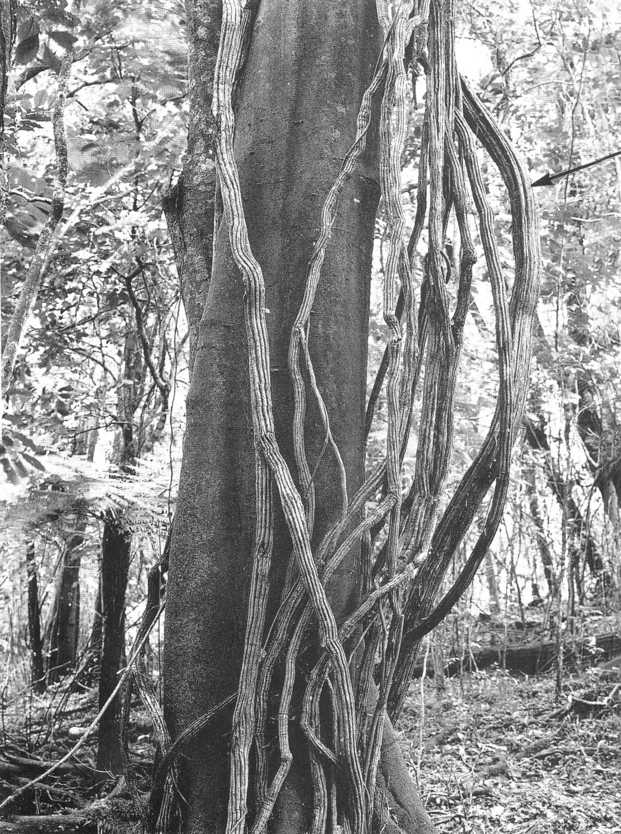
\includegraphics[width=\textwidth]{graphics/figure47puka-roots.jpg}
			\caption[Roots of puka on tawa]{Roots of \IDX{puka} (\BotanicRef{Griselinia lucida}[Griselinia][lucida]) on \IDX{tawa} (\BotanicRef{Beilschmiedia tawa}[Beilschmiedia][tawa]).
			The arrow indicates the stem of a white climbing \IDX{rata} (\BotanicRef{Metrosideros perforata}[Metrosideros][perforata]).
			Paraparaumu, southern North Island.
			Photo: M. D. King.}%
			\label{fig:47puka-roots}
		\end{minipage}
	\end{minipage}
\end{figure}

Generally, when the root tips reach the ground, one main vertical root enlarges greatly until it attains a diameter of \SI{10}{\centi\metre} or more.
This main root usually has a few major branches near the ground and the whole system has a very distinctive appearance resulting from the more or less continuous and pronounced longitudinal grooves and ridges of the bark\figureref{\fullref{fig:46puka-roots}, \fullref{fig:47puka-roots}}.
In its upper parts the main root gives rise to slender, horizontal, girdling roots\figureref{\fullref{fig:48puka-roots}}, which often encircle the trunk of the supporting tree many times and so ensure that the \IDX{puka} will not be dislodged even by the strongest gale.

\begin{figure}[htb]
	% Outer minipage scaled to limit width.
	% Inner minipages scaled so the images have the same height.
	\begin{minipage}[t]{0.9\textwidth}
		\begin{minipage}[t]{(\textwidth-\fgap) * \real{0.422}}
			\centering
			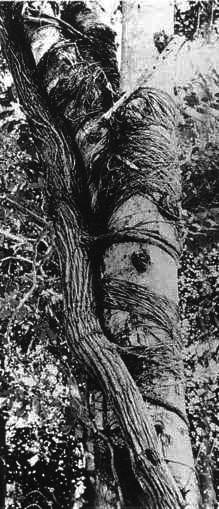
\includegraphics[width=\textwidth]{graphics/figure48puka-roots.jpg}
			\caption[Puka (\emph{Griselinia lucida}) showing girdling roots]{\IDX{Puka}[puka] (\BotanicRef{Griselinia lucida}[Griselinia][lucida]) showing girdling roots.
			Waikanae, southern North Island.
			Photo: M. D. King.}%
			\label{fig:48puka-roots}
		\end{minipage}\hspace{\fgap}%
		\begin{minipage}[t]{(\textwidth-\fgap) * \real{0.578}}
			\centering
			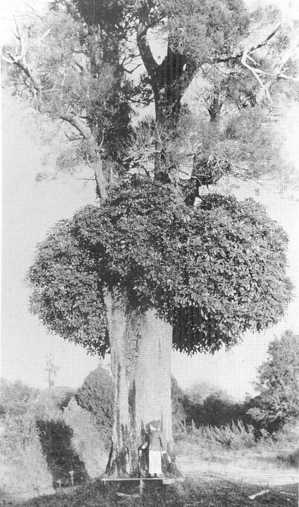
\includegraphics[width=\textwidth]{graphics/figure49fivefinger.jpg}
			\caption[Mountain five-finger on a kahikatea]{Mountain \IDX{five-finger} (\BotanicRef{Pseudopanax colensoi}[Pseudopanax][colensoi]) on a \IDX{kahikatea}.
			National Park, central North Island.
			Photo: J. W. Dawson.}%
			\label{fig:49fivefinger}
		\end{minipage}
	\end{minipage}
\end{figure}

Two other species, \BotanicRef{Griselinia littoralis}[Griselinia][littoralis] and \BotanicRef{Pseudopanax colensoi}[Pseudopanax][colensoi], although mostly terrestrial, can grow as epiphytes in the moist montane or higher latitude forests they favour.
When growing as epiphytes they are generally beyond the altitudinal or latitudinal range of asteliad nests and so establish in the moss and lichen cushions of branch forks.
Like the \IDX{puka}, they eventually send one or more roots to the ground.

Broadleaf (\BotanicRef{Griselinia littoralis}[Griselinia][littoralis]) is the only other species of its genus in New Zealand.
Its leaves are smaller than those of \IDX{puka}, yellowish green and symmetrical or only slightly asymmetrical at the base.
In \IDX{puka}, however, the leaf base is very asymmetrical as the two parts of the leaf divided by the midrib are of quite different lengths.
Broadleaf has been observed as an epiphyte on a variety of trees.
Its descending roots are often more massive than those of \IDX{puka}, but they are not grooved.
The species ranges throughout New Zealand including Fiordland.
Beyond New Zealand \BotanicRef{Griselinia} is found only in Chile, where there are five species, at least some of which are epiphytes.

\IDX{Mountain five-finger}[five-finger!mountain] (\BotanicRef{Pseudopanax colensoi}[Pseudopanax][colensoi]) also has a wide range, but is absent north of \ang{36}S and from Fiordland.
I have observed it growing as an epiphyte on kaikawaka or mountain cedar (\BotanicRef{Libocedrus bidwillii}[Libocedrus][bidwillii]) on Mt.
Taranaki (Egmont) and on \IDX{kahikatea} (\BotanicRef{Dacrycarpus dacrydioides}[Dacrycarpus][dacrydioides]) on the volcanic plateau near Mt.
Ruapehu\figureref{\fullref{fig:49fivefinger}}.

The descending roots of \IDX{puka} and \IDX{mountain five-finger}[five-finger!mountain] seem too slender in relation to their height to stand alone when the supporting trees die, but this may be possible for the more massive roots of the broadleaf.

\subsection{Tree or Strangling Epiphytes}

\begin{figure}[!htb]
	% Outer minipage scaled to limit width.
	% Inner minipages scaled so the images have the same height.
	\begin{minipage}[t]{\textwidth}
		\begin{minipage}[t]{(\textwidth-\fgap) * \real{0.54}}
			\centering
			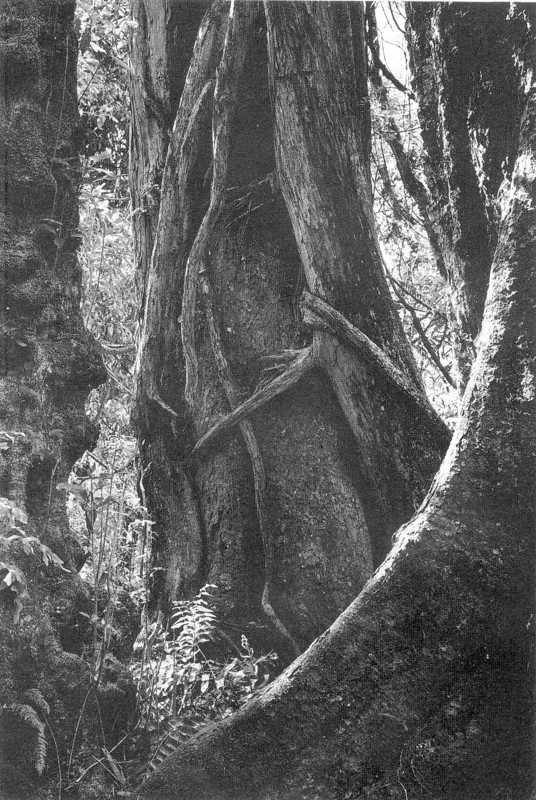
\includegraphics[width=\textwidth]{graphics/figure50rata.jpg}
			\caption[Descending roots and a few girdling roots of the epiphyte northern rata]{Descending roots and a few girdling roots of the epiphyte \IDX{northern rata}[rata!northern] (\BotanicRef{Metrosideros robusta}[Metrosideros][robusta]).
			Te Marua, near Wellington.
			Photo: M. D. King.}%
			\label{fig:50rata}
		\end{minipage}\hspace{\fgap}%
		\begin{minipage}[t]{(\textwidth-\fgap) * \real{0.46}}
			\centering
			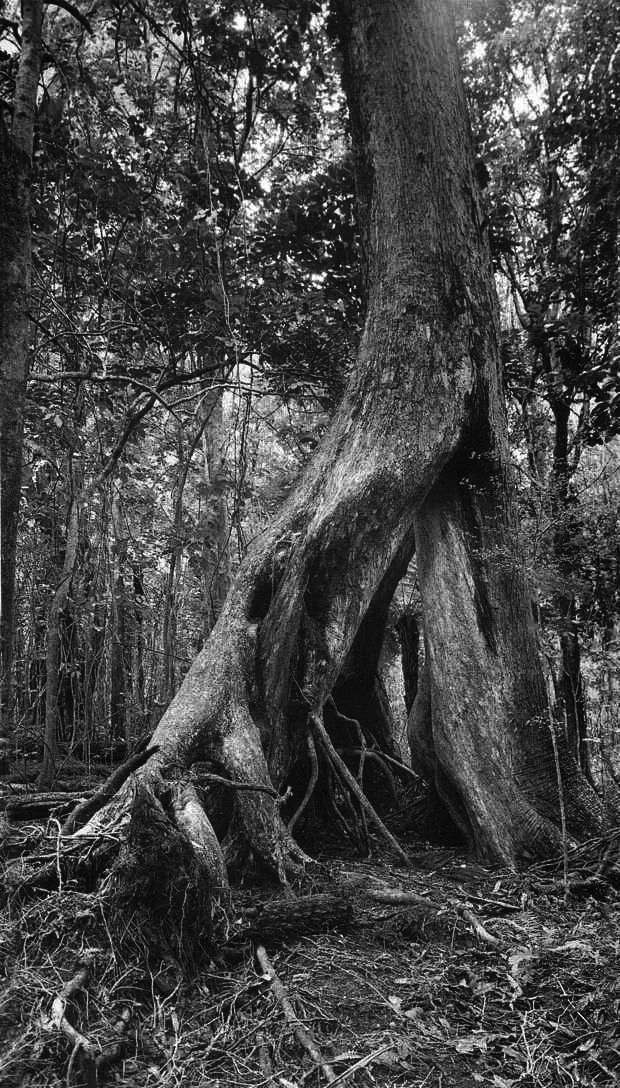
\includegraphics[width=\textwidth]{graphics/figure51rata.jpg}
			\caption[Mature northern rata with a tripod based trunk-like root]{Mature \IDX{northern rata}[rata!northern] (\BotanicRef{Metrosideros robusta}[Metrosideros][robusta]) with a tripod based trunk-like root.
			The original supporting tree is no longer present.
			Paraparaumu, southern North Island.
			Photo: M. D. King.}%
			\label{fig:51rata}
		\end{minipage}
	\end{minipage}
\end{figure}

\IDX{Northern rata}[rata!northern] (\BotanicRef{Metrosideros robusta}[Metrosideros][robusta])\footnote{\cite{dawson1967growth}} is the most notable and common example here.
It is found in lowland forest throughout the North Island and near the north-west coast of the South Island.
It is much more frequent as an epiphyte than as a ground plant and it prefers the tall emergent conifers as supporting trees.
The earlier stages of its life cycle are very similar to those of the \IDX{puka}.
It usually establishes in asteliad nests, although young plants have been observed attached directly to rough bark.
A distinctive feature of some small \IDX{northern rata}[rata!northern] plants is the development of tuber-like swellings on the roots which, it has been suggested, may serve for water storage.\footnote{\cite{beddie1953root}}
Eventually a root grows down the trunk to the ground giving off horizontal girdling roots at intervals\figureref{\fullref{fig:50rata}}.
Unlike \IDX{puka} this descending root does not remain relatively slender, but gradually enlarges to become a metre or more in diameter.
It is often branched near the ground to form a tripod or tetrapod arrangement\figureref{\fullref{fig:51rata}}.
More complicated patterns develop where several branching roots descend from a \IDX{northern rata}[rata!northern] crown to form complexes several metres in diameter.
In some cases more than one \IDX{rata} may be involved, although this is not easy to determine.

\begin{figure}[!htb]
	% Outer minipage scaled to limit width.
	% Inner minipages scaled so the images have the same height.
	\begin{minipage}[t]{\textwidth}
		\begin{minipage}[t]{(\textwidth-\fgap) * \real{0.536}}
			\centering
			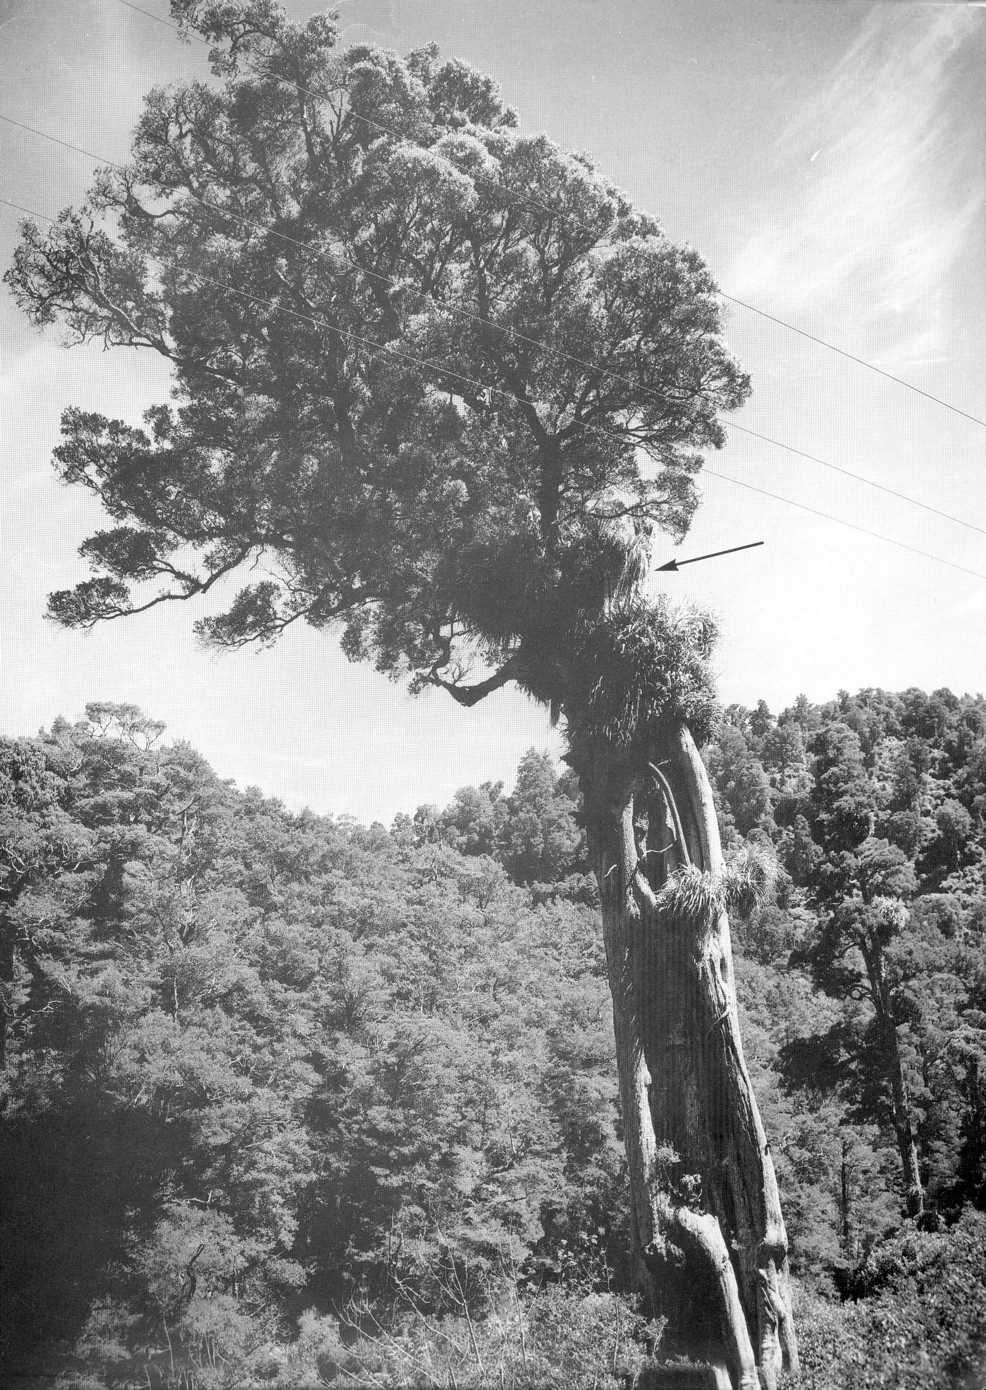
\includegraphics[width=\textwidth]{graphics/figure52rata-branched.jpg}
			\caption[Mature northern rata with a branched trunk-like root system]{Mature \IDX{northern rata}[rata!northern] (\BotanicRef{Metrosideros robusta}[Metrosideros][robusta]) with a branched trunk-like root system.
			The original supporting tree is dead, but its trunk persists inside the \IDX{northern rata}[rata!northern] roots.
			The broken top of the trunk is indicated with an arrow.
			Kaitoke, near Wellington, southern North Island.
			Photo: M. D. King.}%
			\label{fig:52rata-branched}
		\end{minipage}\hspace{\fgap}%
		\begin{minipage}[t]{(\textwidth-\fgap) * \real{0.464}}
			\centering
			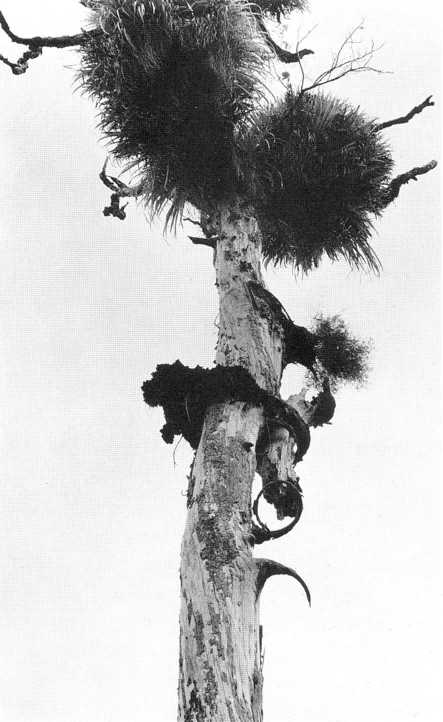
\includegraphics[width=\textwidth]{graphics/figure53dead-rata.jpg}
			\caption[Dead northern rata `trunk' root]{Dead \IDX{northern rata}[rata!northern] `trunk' root, one of whose girdling roots still clasps a portion of the trunk of the original supporting tree.
			The smaller epiphytes are still living showing that they are not parasites as they are clearly not dependent on their tree supports for nutriment.
			Kaitoke, near Wellington, southern North Island.
			Photo: M. D. King.}%
			\label{fig:53dead-rata}
		\end{minipage}
	\end{minipage}
\end{figure}

With the development of such a massive root system, when the supporting tree eventually dies the \IDX{northern rata}[rata!northern] is able to stand alone on its `pseudo-trunk'\figureref{\fullref{fig:52rata-branched}, \fullref{fig:53dead-rata}}.
If the support was an emergent then the \IDX{rata} now replaces it in that role.

The \IDX{northern rata}[rata!northern] and some tropical epiphytic trees of similar habit are often referred to as `stranglers'.
This implies that these epiphytes kill the supporting trees by compressing their trunks within a complete or partial network of roots.
Popular writers on New Zealand plants have taken enthusiastically to this idea, describing the \IDX{northern rata}[rata!northern] variously as a `predatory gangster', `forest bandit' or `notorious strangler' which `crushes', `smothers', `stifles', or `squeezes' the supporting tree in an `iron', `deadly' or `fatal' embrace.\footnote{\cite{druce1971uncle}}

Partly as a reaction to these verbal flights, some botanists in recent times have tended to take a contrary view.\footnote{\cite{zotov1948rata}}
They point out that the light-demanding \IDX{northern rata}[rata!northern] generally establishes in the well lit crowns of mature trees so that, by the time the \IDX{rata} is large enough to stand alone, the supporting tree might well have died of old age.
It does seem, however, that the \IDX{northern rata}[rata!northern] must have some deleterious effect on the supporting tree through partial overshading, root competition, and perhaps in cases where the supporting trunk becomes enlarged within a well developed \IDX{rata} root cage, through some restriction in the movement of water and nutrients.

Recently a distinctive new tree species of \BotanicRef{Metrosideros} (\BotanicRef{Metrosideros bartlettii}[Metrosideros][bartlettii]) has been described.\footnote{\cite{dawson1985metrosideros}}
It is restricted to a few forest patches near North Cape and is similar in epiphytic habit to \IDX{northern rata}[rata!northern].

\IDX{Southern rata}[rata!southern] (\BotanicRef{Metrosideros umbellata}[Metrosideros][umbellata]) is rare and localised in the North Island, but quite common in montane and higher latitude lowland forests in the west of the South Island.
It is mostly terrestrial, but has been observed growing as a `strangling' epiphyte in several places.
Similar \BotanicRef{Metrosideros} epiphytes are known in \IDX{New Caledonia}, Fiji and Hawai{\okina}i.

\section[Epiphytes on Tree Ferns]{Epiphytes on Tree Ferns\thinspace\footnote{\cite{pope1924role}}}

We will consider these separately, as tree ferns provide a substrate rather different from the bark of ordinary trees.
To begin with, tree ferns do not branch so only the trunk is available for colonisation.
Secondly, the trunks are built up from persistent leaf bases and adventitious roots, which provide a variety of surfaces according to the species, but none is quite like bark.
Also the large crowns of leaves cast considerable shade so any epiphytes need to be shade tolerant, at least when young.

The different species of tree fern vary in their suitability for epiphytes.
In our largest and most handsome species, the \IDX{mamaku} (\BotanicRef{Cyathea medullaris}[Cyathea][medullaris]) which has trunks up to \SI{20}{\metre} high and jet-black leaf stalks, the leaf bases decay down to hard leaf scars which collectively form an armour-like surface unsuitable for epiphytes.
In the lower parts of the trunks masses of slender roots grow out, adding considerably to the diameter of the trunk, and these too form a hard dry surface.
The related gully tree fern (\BotanicRef{Cyathea cunninghamii}[Cyathea][cunninghamii]) has similar trunk characteristics.

\begin{SCfigure}[2.0][htb]
	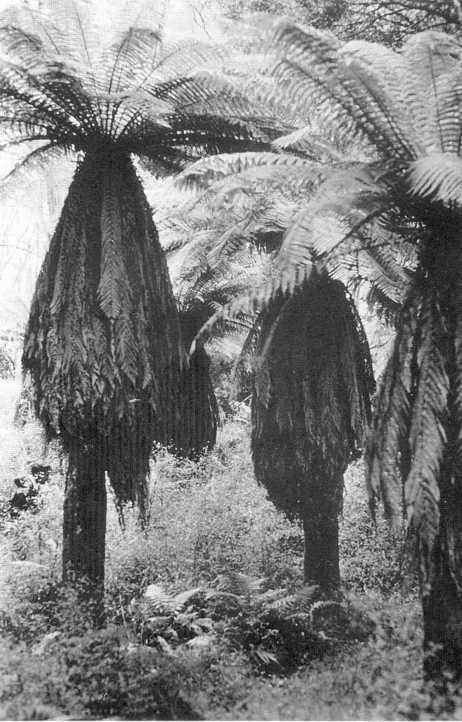
\includegraphics[width=0.66\textwidth]{graphics/figure54dicksonia-fibrosa.jpg}
	\centering
	\caption[\emph{Dicksonia fibrosa} tree ferns with thick `skirts' of dead fronds and stout trunks]{\BotanicRef{Dicksonia fibrosa}[Dicksonia][fibrosa] tree ferns with thick `skirts' of dead fronds and stout trunks, most of whose bulk is made up by interwoven wiry roots.
	Inland Taranaki.
	Photo: J. W. Dawson.}%
	\label{fig:54dicksonia-fibrosa}
\end{SCfigure}

In the \IDX{ponga} or silver tree fern (\BotanicRef{Cyathea dealbata}[Cyathea][dealbata]) the leaf bases decay more gradually and do not form well defined scars.
As a consequence, soil forms readily in the interstices and a variety of epiphytes are able to establish.
\IDX{Wheki}[wheki] (\BotanicRef{Dicksonia squarrosa}[Dicksonia][squarrosa]) has a trunk surface similar to that of the \IDX{ponga}.
In \BotanicRef{Dicksonia fibrosa}[Dicksonia][fibrosa]\figureref{\fullref{fig:54dicksonia-fibrosa}}, \BotanicRef{Cyathea smithii}[Cyathea][smithii] and young plants of \BotanicRef{Cyathea medullaris}[Cyathea][medullaris] and \BotanicRef{Cyathea cunninghamii}[Cyathea][cunninghamii],  epiphytes are discouraged in the upper part of the trunk by the persistence of the old leaves as a `skirt'.\footnote{\cite{page1986tree}}
Thus epiphytes are most commonly found on the trunks of \IDX{ponga} and \IDX{wheki}.

In moist situations, lichens, mosses, liverworts and smaller and larger filmy ferns may be abundant on tree fern trunks.
Climbing \IDX{rata}s and other climbers may also be present as well as a range of seedlings of trees and shrubs which die before reaching maturity.
Here we will consider only the consistent and specialised vascular tree fern epiphytes.
It is worth noting that the species concerned are different in the main from those occurring on ordinary trees.

\subsection{Herbaceous Species}

A lycopodium is quite commonly enountered which is smaller than \BotanicRef{Lycopodium varium}[Lycopodium][varium], and with the leaves associated with the sporangia towards the branch tips often not reduced to scales.
Some treat this lycopodium as a distinct species, \BotanicRef{Lycopodium novae-zelandicum}[Lycopodium][novae-zelandicum]; others regard it as a form of \BotanicRef{Lycopodium varium}[Lycopodium][varium].

\BotanicRef{Asplenium flaccidum}[Asplenium][flaccidum], common on trees, also inhabits tree fern trunks.
The filmy ferns \BotanicRef{Hymenophyllum lyallii}[Hymenophyllum][lyallii], \BotanicRef{Hymenophyllum ferrugineum}[Hymenophyllum][ferrugineum] and \BotanicRef{Trichomanes venosum}[Trichomanes][venosum] are almost confined to tree fern trunks and others are frequently present.
Several species of \BotanicRef{Tmesipteris} remain largely restricted to such sites --- \BotanicRef{Tmesipteris elongata subsp.\ elongata}[Tmesipteris][elongata subsp.\ elongata] throughout and \BotanicRef{Tmesipteris lanceolata}[Tmesipteris][lanceolata] and \BotanicRef{Tmesipteris sigmatifolia}[Tmesipteris][sigmatifolia] in the northern North Island.

\subsection{`Stranglers'}

One shrub and one tree frequently, and several other species less commonly, play this role on tree ferns.

\IDX{Five-finger}[five-finger] (\BotanicRef{Pseudopanax arboreus}[Pseudopanax][arboreus]) is common as a terrestrial plant in shrubby forest regrowth, but in more mature forest it can be surprisingly frequent as a tree fern epiphyte, mostly on the ponga\figureref{\fullref{fig:55fivefinger}}, but also on \IDX{wheki}.
The seedlings establish at the top of the trunk and, being fairly light-demanding, their leaves soon push between and above the fern fronds.
The primary root begins to grow down to the ground, but soon gives off a branch root which grows horizontally around the trunk, sometimes returning to and fusing with the vertical root.
It is thus comparable with the girdling roots of the \IDX{puka} and \IDX{northern rata}[rata!northern].
The vertical root eventually reaches the ground and sometimes branches to enclose the tree fern trunk in a network of roots near the ground.
In the meantime, the crown of the \IDX{five-finger} has continued to branch and grow upward with the tree fern crown following behind it.
\IDX{Raukawa}[raukawa] (\BotanicRef{Pseudopanax edgerleyii}[Pseudopanax][edgerleyii]) and \BotanicRef{Coprosma grandifolia}[Coprosma][grandifolia] may adopt a similar life style but less frequently.

\begin{figure}[htb]
	% Outer minipage scaled to limit width.
	% Inner minipages scaled so the images have the same height.
	\begin{minipage}[t]{\textwidth}
		\begin{minipage}[t]{(\textwidth-\fgap) * \real{0.515}}
			\centering
			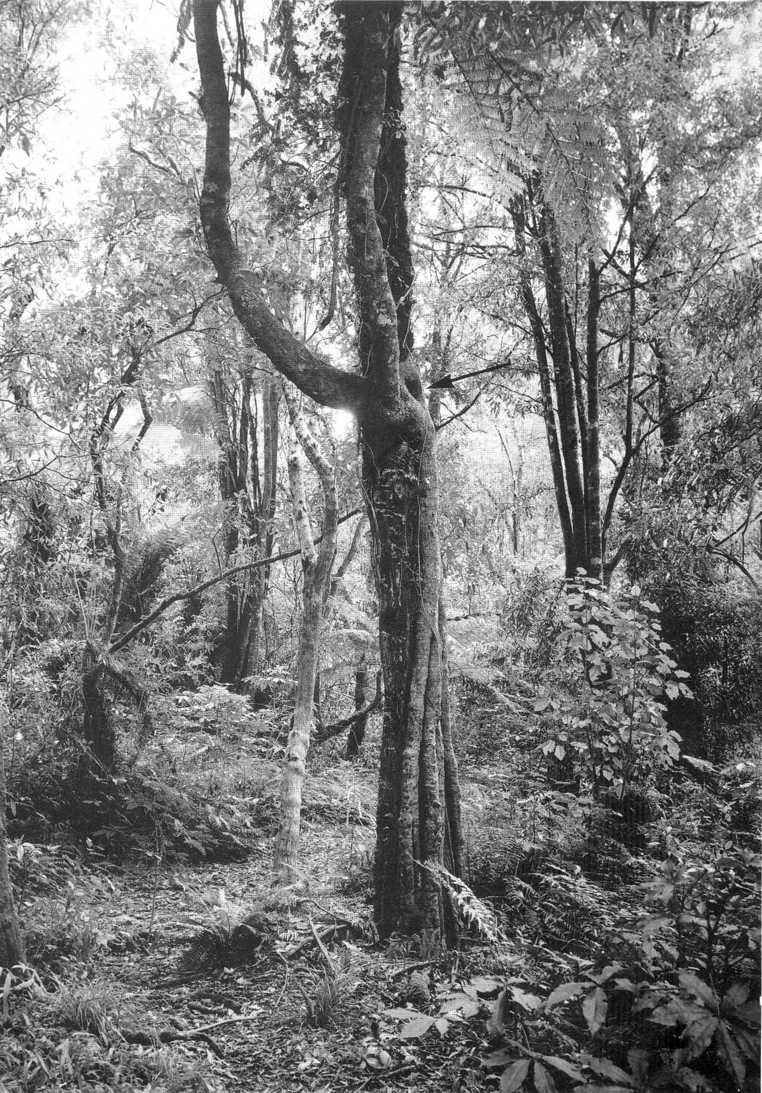
\includegraphics[width=\textwidth]{graphics/figure55fivefinger.jpg}
			\caption[Five-finger epiphytic on a tree fern]{Five-finger (\BotanicRef{Pseudopanax arboreus}[Pseudopanax][arboreus]) epiphytic on a tree fern (\BotanicRef{Cyathea dealbata}[Cyathea][dealbata]). The root/stem junction of the \IDX{five-finger} is indicated with an arrow. Te Marua. Photo:  M. D. King.}%
			\label{fig:55fivefinger}
		\end{minipage}\hspace{\fgap}%
		\begin{minipage}[t]{(\textwidth-\fgap) * \real{0.485}}
			\centering
			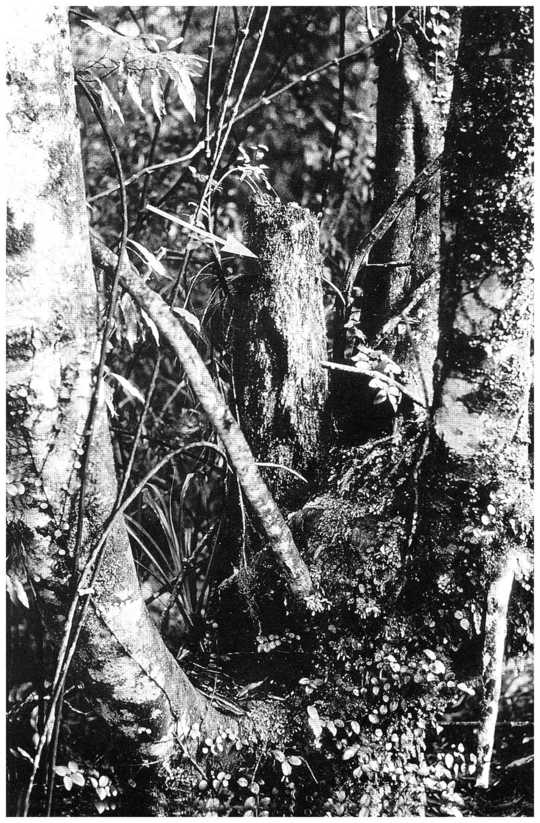
\includegraphics[width=\textwidth]{graphics/figure56kamahi.jpg}
			\caption[Multi-trunked kamahi]{Multi-trunked \IDX{kamahi} (\BotanicRef{Weinmannia racemosa}[Weinmannia][racemosa]), with the base of the tree fern on which it is established indicated by an arrow.
			Photo: J. W. Dawson.}%
			\label{fig:56kamahi}
		\end{minipage}
	\end{minipage}
\end{figure}

\IDX{Kamahi}[kamahi] (\BotanicRef{Weinmannia racemosa}[Weinmannia][racemosa]), the canopy dominant in many montane and higher latitude forests, also frequently begins its life as a tree fern epiphyte, particularly on \IDX{wheki} (\BotanicRef{Dicksonia squarrosa}[Dicksonia][squarrosa]).
In this case the seedlings establish anywhere on the trunks but usually lower down than \IDX{five-finger}.
The \IDX{kamahi} sends a root to the ground, which branches several times but it doesn't seem to form girdling roots.
Instead it often sends a branch root vertically upwards within the tree fern trunk.
The tree fern continues to grow for a time, but eventually breaks off above the junction with the \IDX{kamahi}, leaving a stump.
This stump can often still be discerned among the several spreading trunks of quite large kamahis\figureref{\fullref{fig:56kamahi}}.
In the north of the North Island \BotanicRef{Weinmannia silvicola}[Weinmannia][silvicola] and \BotanicRef{Ackama rosifolia}[Ackama][rosifolia] may also start their lives as low epiphytes on tree ferns.

\section{Epiphytes Growing on Rocks}

As has already been mentioned, epiphytes sometimes grow on the ground and in some circumstances may be important components of terrestrial communities For example on Rangitoto Island, a volcanic cone only a few centuries old in Auckland Harbour, the epiphytes \IDX{northern rata}[rata!northern] (\BotanicRef{Metrosideros robusta}[Metrosideros][robusta]), \IDX{puka} (\BotanicRef{Griselinia lucida}[Griselinia][lucida])\BotanicRef{Brachyglottis kirkii}[Brachyglottis][kirkii] (Senecio),  \BotanicRef{Astelia solandri}[Astelia][solandri] and \BotanicRef{Collospermum hastatum}[Collospermum][hastatum] are common on dry sunny mounds of scoria.
\IDX{Pohutukawa}[pohutukawa] (\BotanicRef{Metrosideros excelsa}[Metrosideros][excelsa]) is also present and it hybridises freely with \IDX{northern rata}[rata!northern].
Further to the south near Wellington there is a remarkable series of raised beaches where on rocky outcrops a number of normally epiphytic orchids are to be found --- \BotanicRef{Earina autumnalis}[Earina][autumnalis], \BotanicRef{Earina mucronata}[Earina][mucronata], \BotanicRef{Dendrobium cunninghamii}[Dendrobium][cunninghamii], and \BotanicRef{Bulbophyllum pygmaeum}[Bulbophyllum][pygmaeum]. \BotanicRef{Drymoanthus adversus}[Drymoanthus][adversus] was also recorded early this century, but seems to have disappeared.
The ferns \BotanicRef{Asplenium flaccidum}[Asplenium][flaccidum] and \BotanicRef{Pyrrosia serpens}[Pyrrosia][serpens] are also present.

\section{Epiphytes Growing on Leaves}

Epiphyllae, as they are termed, are not so evident on the generally smaller leaves of the New Zealand rain forest as they are on the large leaves of the tropical rain forest.
However, in the tropics, the plants concerned are mostly filamentous algae, leafy liverworts and lichens.

One epiphyllous alga in New Zealand is commonly observed on the leaves of \IDX{mahoe} (\BotanicRef{Melicytus ramiflorus}[Melicytus][ramiflorus]).
This is a species of \BotanicRef{Trentepohlia} and it forms conspicuous reddish patches on old leaves of \IDX{mahoe} in autumn and winter.

Twelve epiphyllous species of liverwort in nine genera have been recorded in New Zealand.
They are related to epiphyllae of the tropics and in New Zealand they have been found mostly on fern leaves, but also on leaves of trees and shrubs including \IDX{horopito} (\BotanicRef{Pseudowintera}).

Epiphyllous lichens were the subject of a detailed study by Allan\footnote{\cite{zahlbruckner1928epiphyllous}} at Kitchener Park, Feilding.
They were found to be abundant on the leaves of the conifers \IDX{totara} (\BotanicRef{Todocarpus totara}[Todocarpus][totara]), \IDX{matai} (\BotanicRef{Prumnopitys taxifolia}[Prumnopitys][taxifolia]) and \IDX{kahikatea} (\BotanicRef{Dacrycarpus dacrydioides}[Dacrycarpus][dacrydioides]), on \IDX{tawa} (\BotanicRef{Beilschmiedia tawa}[Beilschmiedia][tawa]), \IDX{titoki} (\BotanicRef{Alectryon excelsus}[Alectryon][excelsus]), rama rama (\BotanicRef{Lophomyrtus bullata}[Lophomyrtus][bullata]), the epiphytic orchid \BotanicRef{Earina mucronata}[Earina][mucronata] and the liane \BotanicRef{Metrosideros colensoi}[Metrosideros][colensoi].
The leaves of \IDX{supplejack} (\BotanicRef{Ripogonum scandens}[Ripogonum][scandens]), the species of \BotanicRef{Coprosma}, \BotanicRef{Pittosporum}, \BotanicRef{Hoheria} and \IDX{puka} (\BotanicRef{Griselinia lucida}[Griselinia][lucida]) were free of lichens.
Clearly much still remains to be learnt about leaf epiphytes in New Zealand.

\section[Parasites]{Parasites\thinspace\footnote{\cite{fineran1974parasitic}}}

Although all flowering plant parasites agree in having structures known as haustoria\figureref{\fullref{fig:57mistletoe-haustori}}, which penetrate into the living tissues of the host, they differ quite widely in a number of other respects.
Some are complete parasites as they lack chlorophyll and so are unable to utilise light energy to manufacture sugars.
Others, which have green leaves, make their own organic nutrients and derive from the host mostly water and inorganic nutrients.
Some parasites are attached to roots, others to trunks and branches.

\begin{figure}[htb]
	% Outer minipage scaled to limit width.
	% Inner minipages scaled so the images have the same height.
	\begin{minipage}[t]{\textwidth}
		\begin{minipage}[t]{(\textwidth-\fgap) * \real{0.452}}
			\centering
			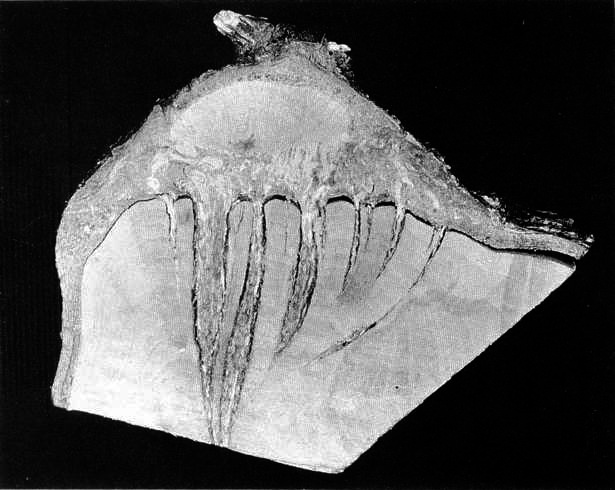
\includegraphics[width=\textwidth]{graphics/figure57mistletoe-haustoria.jpg}
			\caption[Haustoria of a mistletoe]{Haustoria of a mistletoe (\BotanicRef{Peraxilla colensoi}[Peraxilla][colensoi]) penetrating into a branch of \IDX{silver beech}[beech!silver] (\BotanicRef{Nothofagus menziesii}[Nothofagus][menziesii]).
			Photo: J. W. Dawson.}%
			\label{fig:57mistletoe-haustori}
		\end{minipage}\hspace{\fgap}%
		\begin{minipage}[t]{(\textwidth-\fgap) * \real{0.548}}
			\centering
			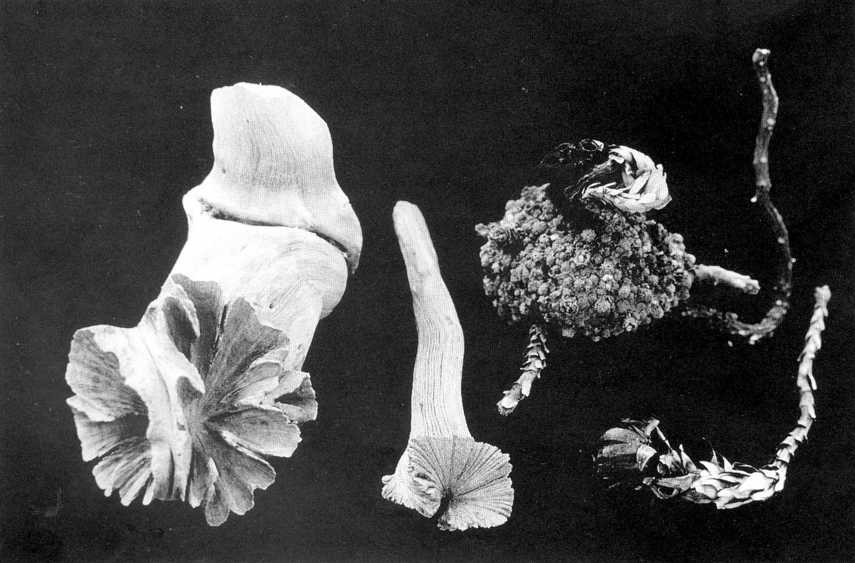
\includegraphics[width=\textwidth]{graphics/figure58dactylanthus.jpg}
			\caption[The root parasite \emph{Dactylanthus taylorii}]{The root parasite \BotanicRef{Dactylanthus taylorii}[Dactylanthus][taylorii].
			On the right is the knobbly plant body of the parasite with a scaly inflorescence as well as a separate inflorescence.
			On the left are `wooden roses' or the distinctive forms of the host roots after the parasites have been removed.
			Photo: J. W. Dawson.}%
			\label{fig:58dactylanthus}
		\end{minipage}
	\end{minipage}
\end{figure}

\section{Root Parasites}

\BotanicRef{Dactylanthus taylorii}[Dactylanthus][taylorii]\footnote{\cite{moore1940structure}}\figureref{\fullref{fig:58dactylanthus}} is a complete parasite attached to the roots of a range of mostly small tree species in lowland to montane forest throughout the North Island.
It is not readily observable as only the reddish-brown, scaly inflorescences appear above the ground.
The strange appearance of the flower heads which apparently arise directly from the ground, led the Maori to give the name te pua o te rēinga (flower of the Underworld) to this species.

Apparently the embryo root of a \BotanicRef{Dactylanthus} seed penetrates the slender root of a suitable host, then gradually expands into a tuber-like structure which eventually surrounds the host root.
The terminal portion of the host root then dies away.
The `tuber' continues to enlarge and the end of the host root enlarges with it into a disc-like form.
Both can attain a diameter of up to \SI{30}{\centi\metre}.
The tuber has a flattened ball-like shape and is covered with hard warty protuberances.
Inflorescence buds originate between these, bearing male flowers on some plants, female flowers on others.
The flowers have a strong sweet perfume which is attractive to flies.
The junction between host and parasite is not flat, but formed into radiating grooves, v-shaped in section.
It has been found that if the host/parasite mass is boiled, the parasite can be removed exposing the expanded, fluted ends of the host roots.
These `wooden roses', as they are called, are prized as curios. \BotanicRef{Dactylanthus} is restricted to New Zealand but belongs to a largely tropical and subtropical family.

Although \BotanicRef{Mida salicifolia}[Mida][salicifolia]\footnote{\cite{philipson1959some}} is a root parasite on a wide range of trees including \IDX{kauri}, unlike \BotanicRef{Dactylanthus} it does not advertise the fact.
It is a small tree with narrow, green willow-like leaves in one variety and rather broader leaves in the other.
It is found in lowland forests throughout the North Island, but becomes uncommon in the south of its range.
The only other species of the genus is restricted to the Juan Fernandez islands near Chile.

Other root parasites in New Zealand are found in open subalpine and alpine sites. \BotanicRef{Exocarpus bidwillii}[Exocarpus][bidwillii] is leafless with stiff, yellow-green stems branching in a coral-like fashion.
Other species of the genus are small trees and shrubs of the tropics (Madagascar, Australia, Malaysia, \IDX{New Caledonia}, Polynesia).

Like \BotanicRef{Mida}, the fifteen green-leaved, mostly alpine herbs of the genus \BotanicRef{Euphrasia}\footnote{\cite{philipson1959some}} in New Zealand give no hint of their parasitic behaviour.
The genus is widespread in temperate regions of both hemispheres.

\section{Branch Parasites}

These all contain chlorophyll so are only partly dependent on their hosts for organic nutrients.
All but one of the New Zealand parasites in this category belong to two largely tropical families --- Viscaceae and Loranthaceae, collectively referred to as mistletoes.
In the first the flowers are small and inconspicuous, in the second they are much larger and often brilliantly coloured.

Three small species of \BotanicRef{Korthalsella} represent the Viscaceae.
All have vestigial leaves and strongly jointed stems, which in \BotanicRef{Korthalsella lindsayi}[Korthalsella][lindsayi] and \BotanicRef{Korthalsella clavata}[Korthalsella][clavata] are strongly flattened and in \BotanicRef{Korthalsella salicornioides}[Korthalsella][salicornioides], cylindrical. \BotanicRef{Korthalsella salicornioides}[Korthalsella][salicornioides] is found throughout the country while \BotanicRef{Korthalsella lindsayi}[Korthalsella][lindsayi] and \BotanicRef{Korthalsella clavata}[Korthalsella][clavata] are found from the central North Island southwards.
Both parasitise a wide range of shrubs and small trees.

The New Zealand species in the family Loranthaceae are all green-leaved, freely branching shrubs of up to one metre in diameter.
Currently all these species are referred to a number of small genera,\footnote{\cite{barlow1966revision}} with one exception endemic to New Zealand, although formerly some were included in the tropical genera \BotanicRef{Elytranthe} and \BotanicRef{Loranthus}.  \BotanicRef{Tupeia antarctica}[Tupeia][antarctica] is the only species of a genus restricted to New Zealand.
Each plant is attached to a ball-like mass, which is a combination of the parasite haustorium and the host tissues. \BotanicRef{Tupeia} is found throughout the country and attacks a wide range of both native and introduced shrubs and small trees, and occasionally other branch parasites.

\BotanicRef{Peraxilla colensoi}[Peraxilla][colensoi] and \BotanicRef{Peraxilla tetrapetala}[Peraxilla][tetrapetala] mostly parasitise \BotanicRef{Nothofagus} species in both islands.
They have bright red flowers which form eye-catching patches of colour against the dark green beech foliage.
The orange flowers of \BotanicRef{Alepis flavida}[Alepis][flavida], seen mostly on beech trees, are also very attractive. \BotanicRef{Trilepidea adamsii}[Trilepidea][adamsii], with reddish cream flowers, is restricted to the northern Coromandel Peninsula and adjacent localities and was last recorded in the 1960s. \BotanicRef{Ileostylus micranthus}[Ileostylus][micranthus] has small green flowers and yellow berries.
It is widespread in New Zealand and Norfolk Island and has as its hosts a range of shrubs, small trees and, sometimes, conifers both native and introduced.
The species of all these genera except \BotanicRef{Tupeia} send out roots over the bark surface which form secondary haustoria at intervals. \BotanicRef{Ileostylus} alone can form new leafy shoots from its roots.

The branch parasites have berries which are eaten by birds and the seeds deposited on tree branches.
The seeds are attached to bark by a sticky secretion.
Some branch parasites elsewhere have explosive fruits, which shoot the seeds for several metres.
This has been observed in the New Zealand species of \BotanicRef{Korthalsella}.

\begin{SCfigure}[1][htb]
	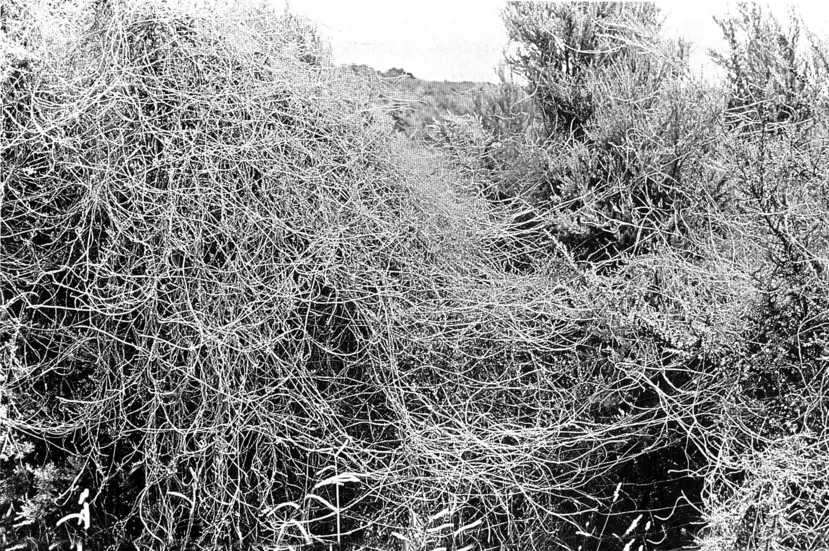
\includegraphics[width=0.66\textwidth]{graphics/figure59cassytha.jpg}
	\centering
	\caption[Tangled thread-like stems of the leafless parasite \emph{Cassytha pubescens}]{Tangled thread-like stems of the leafless parasite \BotanicRef{Cassytha pubescens}[Cassytha][pubescens] on \IDX{manuka} (\BotanicRef{Leptospermum scoparium}[Leptospermum][scoparium]).
	Near North Cape, North Island.
	Photo: J. W. Dawson.}%
	\label{fig:59cassytha}
\end{SCfigure}

The remaining parasite in this category is \BotanicRef{Cassytha pubescens}[Cassytha][pubescens].
A twining vine as well as a parasite, it is quite different from the rest.
Its seeds germinate in the ground and the slender yellow green primary stem with rudimentary leaves rotates in anti-clockwise direction winding tightly around any stems it encounters.
At frequent intervals haustoria penetrate the host.
The stems of the \BotanicRef{Cassytha} branch freely, but remain slender, festooning the shrub hosts with tangled stringlike masses\figureref{\fullref{fig:59cassytha}}.
This species is restricted to the northern half of the Northland peninsula where it grows on shrubs and particularly \IDX{manuka} (\BotanicRef{Leptospermum scoparium}[Leptospermum][scoparium]).
It is surprising to find that \BotanicRef{Cassytha} belongs to the Lauraceae, a family which otherwise consists of mostly tropical and subtropical trees including the species of \BotanicRef{Beilschmiedia} and \BotanicRef{Litsea} in New Zealand.
Our species of \BotanicRef{Cassytha} is also found in Australia and there are other species there and in Melanesia, tropical Asia and South Africa.

\section{Saprophytes}

Vascular saprophytes are completely without chlorophyll and are often small, pale plants growing in leaf litter in very shady places in rain forests.
It is thought that they gain their organic nutrients from decaying plant material.
Their underground parts are penetrated by fungal threads and recent studies, some in New Zealand, have shown that in some cases the fungal threads are also attached to the roots of nearby trees.
It has been suggested that such saprophytes, and probably others, may be secondary parasites drawing nutriment from tree roots via fungal threads.\footnote{\cite{campbell1962mycorrhiza}},\footnote{\cite{campbell1968investigation}}

The New Zealand saprophytes are all orchids, except for one belonging to the Burmanniaceae, a family closely related to the Orchidaceae.
This is \BotanicRef{Thismia rodwayi}[Thismia][rodwayi],\footnote{\cite{campbell1968investigation}} which has been found only in the northern half of the North Island, and there mostly on the volcanic plateau.
The pinkish scale-leaved stems, arising from a branching root system, each end in a relatively large delicate flower, which has been likened to a red lantern.
Our species is also found in Tasmania and Victoria and there are other species in Australia, tropical Asia and America.

\BotanicRef{Coryhas cryptanthus}[Coryhas][cryptanthus] is the only saprophyte among the eight New Zealand species of the genus.
It has been collected at scattered localities throughout the country.
Only the flower appears above the leaf mould; the stem then elongates to carry the capsule to about \SI{15}{\centi\metre} above the ground.
The genus ranges from south-east Asia through Australia to New Zealand.

The 15 species of \BotanicRef{Gastrodia} ranging from India and Japan to Australasia are all saprophytes.
The branching underground rhizomes are tuberous and filled with starch; those of the New Zealand species were eaten by the Maori.
The stems are tall, up to \SI{1}{\metre}, and can be attractively if strangely coloured.
They often appear polished, with flecks of white and brown which give a resemblance to wood grain. \BotanicRef{Gastrodia cunninghamii}[Gastrodia][cunninghamii] and \BotanicRef{Gastrodia minor}[Gastrodia][minor] are found throughout, \BotanicRef{Gastrodia cunninghamii}[Gastrodia][cunninghamii], mostly in beech forest, and \BotanicRef{Gastrodia minor}[Gastrodia][minor] mostly under \BotanicRef{Leptospermum}. \BotanicRef{Gastrodia sesamoides}[Gastrodia][sesamoides] has not been discovered further south than \ang{42}S in the South Island and is found in open forest and shrubland.

\BotanicRef{Yoania australis}[Yoania][australis] was only discovered in recent times, but is now known from several localities in \BotanicRef{Beilschmiedia tarairi}[Beilschmiedia][tarairi] forest on the Northland peninsula.
The stems bearing the small flowers are a pale rose colour and up to \SI{20}{\centi\metre} tall.
The genus is entirely saprophytic and is known at several localities in Asia and north Africa.

\section{Conclusion}

In view of its wide range of specialised growth forms and habits, reviewed in this and in the last chapter, it is not difficult to conclude that in these aspects New Zealand conifer broadleaf forest comes closer to tropical rain forest than to any other type of vegetation, despite New Zealand's temperate latitudes.
In the light of certain fossil evidence the most likely explanation for this is that, before the Ice Age, forest of the general type now largely confined to tropical latitudes was also widespread in the middle latitudes of both hemispheres.
Plant fossils from the vicinity of London dating back to early Tertiary times (80 million years ago) belong to genera, including some palms, now largely restricted to the tropics.\footnote{\cite{chandler1964lower}}
Fossil floras with similar relationships have also been discovered in Oregon, U.S.A.
The Ice Age, the effects of which would have been more severe in the largely continental northern hemisphere, virtually eliminated such forests from middle northern latitudes, with the exception of southern Japan and parts of China, while limited examples persisted in middle southern latitudes, and in New Zealand best of all.

Remnants of such middle latitude rain forests, with fewer species than those of New Zealand and in particular fewer vines and epiphytes, can be found in parts of New South Wales and Victoria in Australia, along a portion of the south-east coast of South Africa, and in central Chile.
The rain forests of these areas may have been more reduced than those of New Zealand by the development of arid continental climates and by their longer history of human and natural fires as well as by Ice Age coldness.
New Zealand's narrow oceanic land mass would have ameliorated the two climatic factors and enabled the survival of our fascinating array of vines, epiphytes, parasites and saprophytes.
However, with its fewer species, its relatively small leaves and admixture of conifers the New Zealand conifer broadleaf forest probably comes closest to certain montane tropical rather than lowland tropical rain forests.
The conifer broadleaf forest also shares more genera with the former than with the latter.

Perhaps the New Zealand conifer broadleaf forest and related forest types elsewhere in the southern hemisphere evolved in some degree of isolation on Gondwana.
The presence of certain specialised growth forms, comparable with but unrelated to those of the old and new world tropics (nest epiphytes --- \BotanicRef{Collospermum}, \BotanicRef{Astelia}; hemiepiphytes --- \BotanicRef{Griselinia}, \BotanicRef{Metrosideros}; lianes --- \BotanicRef{Metrosideros} species) lends support to this suggestion.
